\newpage

% Из текста короткого задания на ВКР:
% 1. Проанализировать технологии, используемые для реализации бесконтактного взаимодействия платежного терминала и средства платежа (карты, смартфона и пр.).
% 2. Проанализировать методы и инструменты обеспечения безопасности бесконтактных платежей
% -. Сравнение существующих аналогов систем коррекции
% -. Выбор методы и технологий разработки системы


%  - Как технически выглядит процесс оплаты (от введения суммы и прикладывания карты, до отображения статуса платежа)
%  - Декомпозиция процесса на технологии, используемые на разных этапах
%  - Обзор технологий
%    - с точки зрения тех. процесса
%    - с точки зрения безопасности
%  - Сравнительный анализ существующих решений
%  - Формирование требований к системе (используемые технологии, превосходство над аналогами)

\section{Анализ предметной области}

\subsection{Развитие сферы банковских платежей}

\subsubsection{Развитие платежных операций}

Появление банковской системы, выступающей в качестве посредника между государством и гражданами, ознаменовало процесс непрерывного развития финансовых технологий, поскольку банки стремились повысить свою прибыльность, в том числе путем повышения качества платежных сервисов.
Деньги выступали в качестве основного способа оплаты товаров и услуг, однако не всегда были удобным способом оплаты, поэтому в дополнение к ним сначала появились бумажные чеки, а позднее и банковские карты.
Вместе с появлением банковских карт, появились и платежные системы~-- инстанции, которые не только выпускали и поддерживали карты, но и выступали посредниками между банками.
Для приема карт к оплате необходимы были специальные устройства.
Изначально это были импринтер, с помощью которого создавались слипы~-- бумаги, содержащие реквизиты карты, дату и сумму покупки и др..
Ему на смену пришел электронный терминал оплаты (POS-терминал), который упрощал взаимодействие с картой, т.к. передавал информацию о карте напрямую в процессиноговые центры платежной системы.

При приеме карты кассир должен был получить информацию от банка, что у держателя карты есть необходимый объем денежных средств для оплаты, в противном случае товар или услуга не могла быть оплачена.
Изначально этот процесс выглядел следующим образом: кассир звонил в банк-эквайер, тот связывался с банком-эмитентом, выпустившем карту, который подтверждал наличие необходимой суммы и инициировал ее передачу в банк-эквайер либо сообщал о невозможности оплаты.
Платежные системы изначально выступали каналом связи между банками.
Однако с увеличением количества карт создавалась высокая нагрузка на банки, и с целью ее снижения появились специальные процессинговые центры, которые совместно с платежными системами осуществляли функцию клиринга~\cite{habr_fondy_payment_history}.

Клиринг~-- это комплекс взаиморасчётов за оказанные услуги, проданные товары или ценные бумаги, основанные на безналичных расчётах.
Клиринг в платёжной системе~-- это взаиморасчёты по любым операциям, совершённым с помощью банковской карты.
Функцию клиринга выполняет ПС, за счет нее снижается нагрузка на банки, выступающие в роли эквайеров, т.к. ПС переводит им деньги в конце операционного дня~\cite{habr_nspk_cliring}.

Процесс идентификации голосом постепенно ускорялся, за счет повышения стабильности и качества телефонии.
Однако с ужесточением требованием ПС к времени подтверждения транзакции и развития банковских алгоритмов ему на смену пришла авторизация по пин-коду, которая является актуальной технологией на данный момент.
ПС совместно с банками продолжают развивать технологию авторизации, в результате чего сейчас для выполнения платежных операций, не превышающих определенный лимит, не требуется пин-код.

Также на текущий момент в России активно развивается оплата посредством QR-кодов, предоставляемых Системой Быстрых Платежей (СБП) и/или банками-эквайерами.
Данная технология оказалась востребованной среди пользователей, поскольку для оплаты по QR подойдет любое мобильное устройство с камерой и выходом в интернет.
А после наложения на Россию санкций в 2022-м году смартфоны под управлением ОС IOS лишились возможности оплаты посредством NFC, и оплата по QR-коду стала единственно-возможным вариантом~\cite{habr_nspk_qr}.


\subsubsection{Развитие банковских карт}

Банковские карты так же, как и сами платежные операции, претерпели ряд изменений.
Сначала в них появилась магнитная полоса для быстрой идентификации карты платежным терминалам с помощью статических данных, хранимых в карте.
В 1993 году международные платёжные системы Mastercard, Visa и Europay подписали соглашение о совместной работе, чтобы развить технологии банковских карт.
В результате чего в 1994 году была выпущена первая версия стандарта EMV и систем на его основе.

Данный стандарт предусматривал наличие специального EMV-чипа, встроенного в карты.
Данный чип~--- это микропроцессор, предназначенный для безопасного хранения и обработки данных при проведении платежных операций.
В отличие от традиционной магнитной полосы, которая содержит статичные данные и легко подделывается, EMV-чип генерирует уникальный криптографический код для каждой транзакции, что делает её практически невозможной для подделки~\cite{emv_specifications_book}.

EMV-стандарт был внедрен с целью глобального повышения безопасности безналичных платежей и снижения уровня подделки карт и кражи их данных.
EMV-стандарт ввел понятие офлайн транзакции~-- платежной операции исключительно с участием карты и платежного терминала, которые проводит ее офлайн аутентификацию.
В онлайн транзакции терминал связывается в режиме реального времени с банком-эквайером, который через ПС запрашивает аутентификацию карты у банка-эмитента.

После массового внедрения EMV-карт во многих странах наблюдалось значительное снижение случаев фрода с использованием поддельных карт~\cite{plas_emv_fraud}.
Фрод~-- это проведение мошеннических (неправомерных) операций с использованием банковских карт.
Кроме того, EMV-чип лег в основу технологий бесконтактной оплаты, таких как PayPass (Mastercard), payWave (Visa) и Mir Accept (НСПК), где также используется принцип одноразовых криптограмм.
Бесконтактные карты используют технологию радичастотной модуляции сигнала (RFID), с использованием антенны, встроенной в карту, представленной на рисунке~\ref{fig:emv_card}.

\begin{figure}[H]
    \centering
    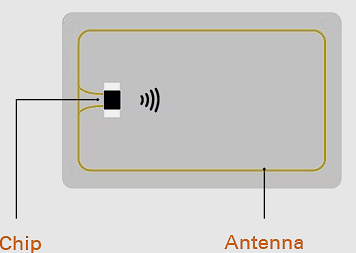
\includegraphics[width=0.4\textwidth]{images/research/emv_card}
    \caption{\centering Структура бесконтактной EMV-карты}
    \label{fig:emv_card}
\end{figure}

С распространением технологии NFC появилась сфера мобильных платежей.
Покупатели получили возможность быстро и безопасно выполнять оплату посредством устройств с поддержкой NFC с помощью виртуальных карт, добавленных в приложение «цифрового кошелька».
Примеры подобных приложений: Apple Pay, Google Pay, Mir Pay и др..



\subsection{Анализ процесса платежа через терминал}
\label{subsec:payment_process}

\subsubsection{Оплата бесконтактной картой}
\label{subsubsec:contactless_payment}

Процесс оплаты с использованием бесконтактной банковской карты может протекать несколькими различными способами.
Как уже было упомянуто ранее, есть онлайн и офлайн оплата через терминал.
Первая происходит с запросом подтверждения банком-эквайера от банка-эмитента в реальном времени.
Вторая происходит исключительно без моментального подтверждения банком, с участием карты и платежного терминала, который проводит ее аутентификацию.
Также для оплаты могут использоваться разные типы карт.
Однако именно бесконтактную оплату поддерживается только картами, соответствующими стандарту EMV.

При этом карта в защищенной области памяти хранит общий с эмитентом ключ MK-AC (Application Cryptogram Master Key).
Во время совершения оплаты при онлайн-операции карта генерирует на основе MK-AC сессионный ключ SK-AC (Application Cryptogram Session Key) и использует его, данные карты и данные об операции, полученные с терминала, для генерации криптограммы операции ARQC (Authorization Request Cryptogram).
В основе генерации криптограммы лежит алгоритм 3DES (Triple DES).
В общем случае данные по операции поступают от карты к платежному терминалу, далее на хост банка-эквайера, затем к платежной системе и на самом последнем этапе к банку-эмитенту для авторизации.
Результат авторизации передается назад на платежный терминал и карту.
Данный процесс изображен на рисунке~\ref{fig:emv_card_payment}.

\begin{figure}[H]
    \centering
    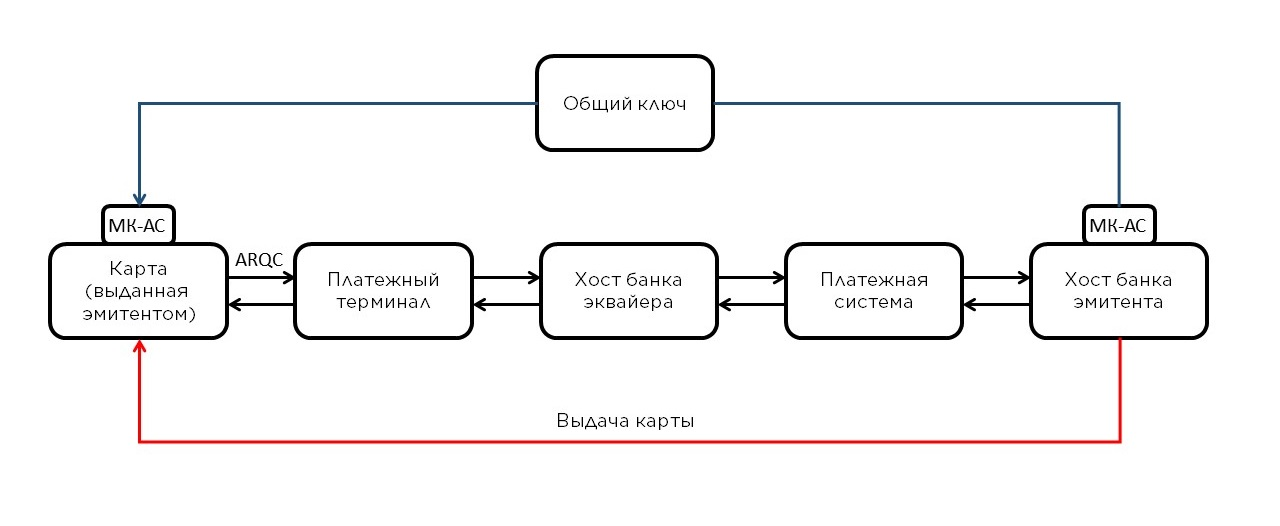
\includegraphics[width=0.8\textwidth]{images/research/emv_card_payment}
    \caption{\centering Процесс оплаты посредством EMV-карты}
    \label{fig:emv_card_payment}
\end{figure}

Банк-эмитент проверяет пришедшую криптограмму операции, путем ее сравнения со значением, которое генерирует сам на основе данных об операции, пришедших вместе с ARQC.
Банк-эмитент может одобрить или отклонить операцию по результатам анализа данных карты, криптограммы, установленных лимитов операций, рисков, а также других параметров~\cite{habr_nspk_mir_payment}.

Далее банк-эмитент на основе динамических данных транзакции генерирует ARPC (Authorisation Response Cryptogram) и отправляет эту криптограмму карте.
В тот момент, когда карта подтвердит пришедший ARPC, взаимная аутентификация карты и эмитента – выполнена~\cite{emv_card_mechanism}.


\subsubsection{Оплата мобильным приложением-кошельком}

При оплате мобильным кошельком выданная банком-эмитентом карта непосредственного участия в оплате не принимает.
Держатель карты вносит данные карты в цифровой кошелек, после чего карта «добавляется» в приложение, точнее не она, а специальный токен-профайл, сгенерированный на базе этой карты.
При этом карточные данные и ключ эмитента MK-AC, хранимый на карте, на телефон не передаются, поэтому оплата посредством приложения происходит с использованием токен-профайла и его специальных ключей.

Процесс добавления карты в приложение-кошелек представлен на рисунке~\ref{fig:add_mob_cardholder}.

\begin{figure}[H]
    \centering
    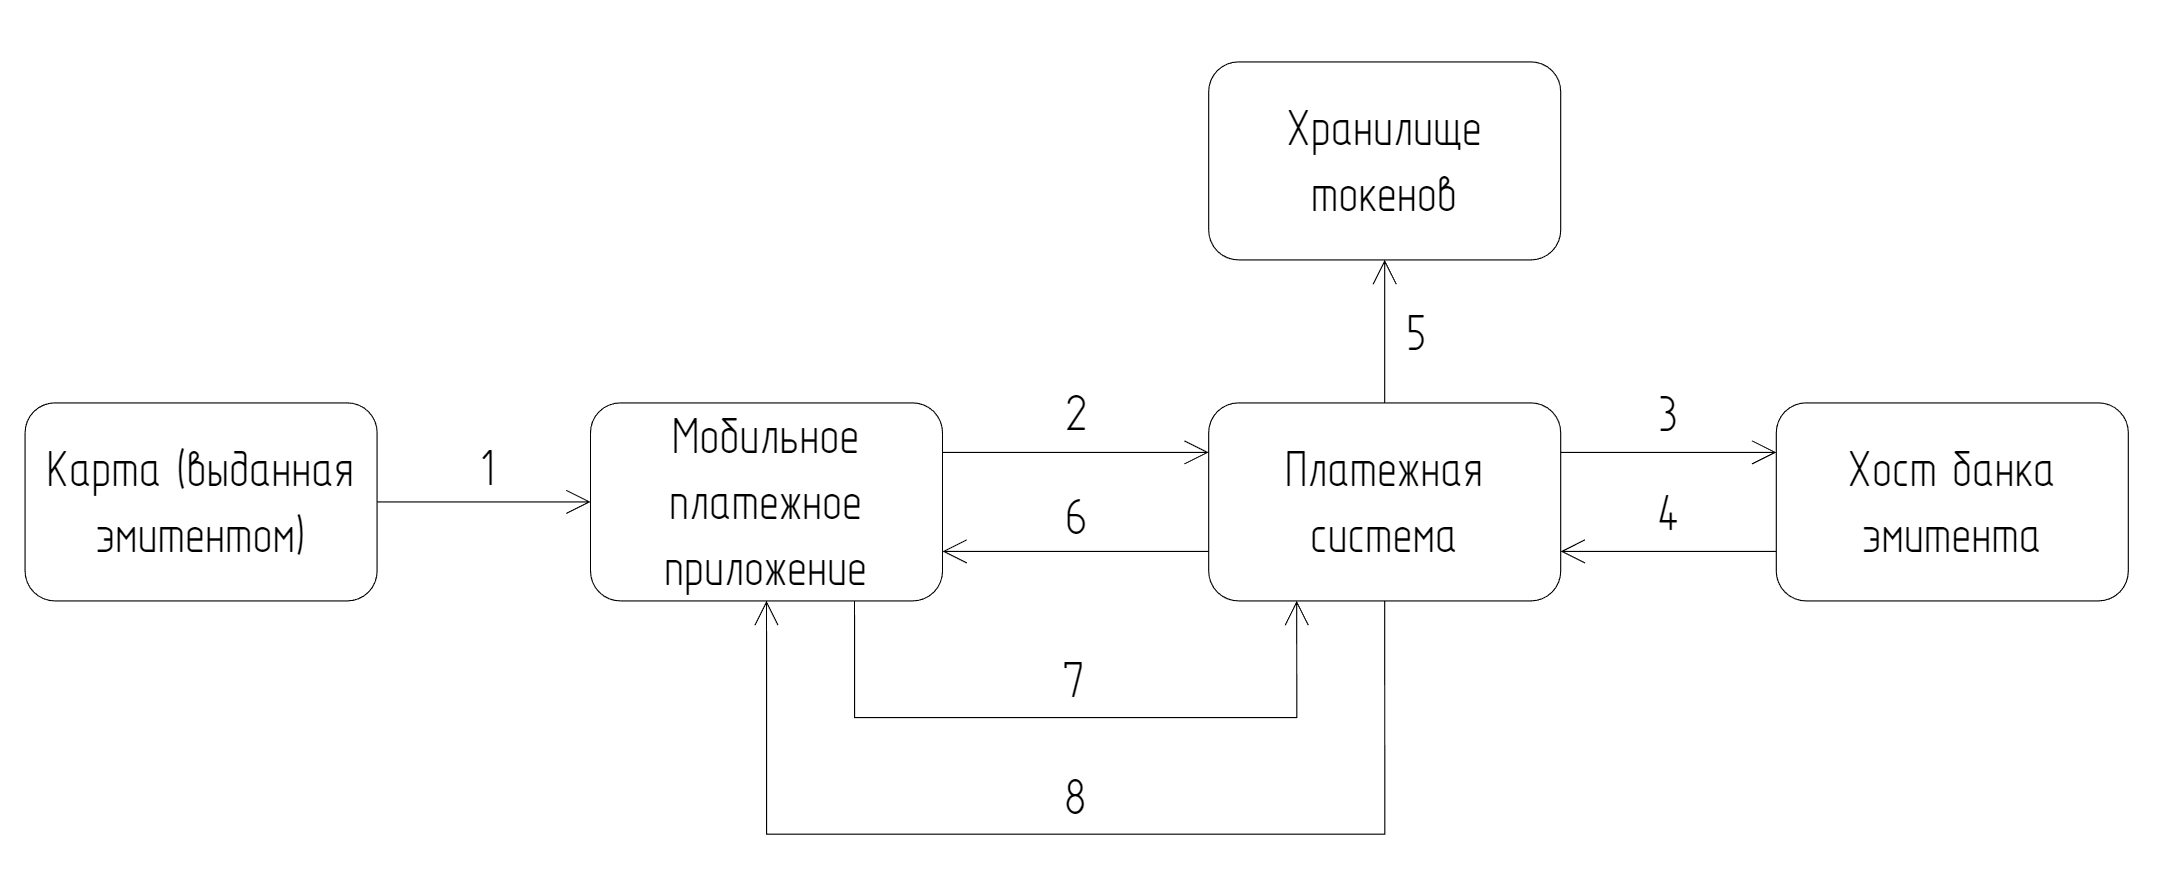
\includegraphics[width=0.8\textwidth]{images/research/add_mob_cardholder}
    \caption{\centering Процесс оплаты посредством мобильного приложения-кошелька}
    \label{fig:add_mob_cardholder}
\end{figure}

Цифрами на рисунке~\ref{fig:add_mob_cardholder} обозначены следующие этапы добавления карты в кошелек:

\begin{enumerate}
    \item держатель карты вводит данные в приложение;
    \item приложение передает их в зашифрованном виде через поставщика услуг мобильного кошелька(WSP~-- Wallet Service Provider) в платежную систему (в случае приложения Mir Pay поставщиком услуг кошелька является НСПК~-- Национальная система платежных карт~-- поэтому данные сразу попадают в ПС);
    \item платформа мобильных платежей (ПМП) производит обработку данных: расшифровывает их, по номеру карты определяет, каким эмитентом она была выдана, и запрашивает у него подтверждение на возможность добавления карты в кошелек;
    \item банк-эмитент возвращает подтверждение или запрет на возможность добавления карты в кошелек;
    \item в случае получения подтверждения для данной карты происходит процедура генерации токен-профайла;
    \item передачи токен-профайла в мобильное приложение пользователя;
    \item мобильное приложение запрашивает у ПМП несколько одноразовых ключей, которые будут использоваться приложением при совершении покупки в качестве сессионных ключей для проведения операции, аналогичных SK-AC.
\end{enumerate}

Таким образом, вместо карточных данных на мобильном устройстве будет храниться токен-профайл, который привязан к конкретным карте и устройству.
Преобразование токен-профайла в исходные данные карты вне платформы мобильных платежей является невозможным.
Одноразовые ключи не могут быть применены более одного раза, поэтому в процессе использования мобильное приложение с некоторой периодичностью подгружает из ПМП новые ключи.


Стоит отметить, что в Mir Pay используется схема, при которой происходит хранение нескольких одноразовых ключей, но существует и другой подход, при котором происходит хранение одного ключа на устройстве.
Такой подход требует наличия аппаратного элементов безопасности (АЭБ) на устройстве, например TEE (Trusted Execution Environment) или SE (Secure Element), и некоторые кошельки применяют именного этот подход, однако он накладывает ограничение в виде наличия АЭБ в устройстве.
Mir Pay также использует АЭБ при его наличии, но уже для хранения одноразовых ключей.

Высокая степень безопасности при использовании приложения гарантируется тем, что для обмена конфиденциальными данными ПМП и Mir Pay генерируют ключевые пары и обмениваются лишь публичными компонентами.
При этом хранением разных ключевых компонент происходит в разных системных хранилищах: как в ключевом хранилище, так и в оперативной памяти.
Для совершения мошеннической операции придется извлечь и расшифровать криптограммы всех ключей, а это неэффективно, в силу того, что для проведения операций используются строго одноразовые ключи.
Передача конфиденциальных данных, например токен-профайла, одноразовых ключей для проведения операций и данных по уже совершенным операциям, начинается только после того, как Mir Pay и ПМП обменялись публичными ключами, создав защищенный канал, и происходит только с использованием <<крипто-стойких>> алгоритмов~\cite{habr_nspk_mir_payment}.

Процесс оплаты с помощью приложения кошелька представлен на рисунке~\ref{fig:emv_mob_payment}.

\begin{figure}[H]
    \centering
    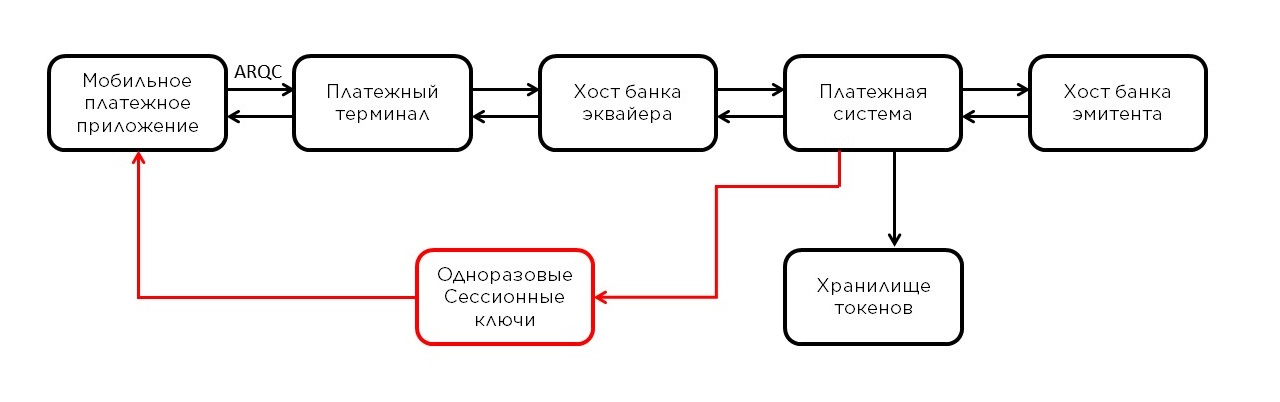
\includegraphics[width=0.8\textwidth]{images/research/emv_mob_payment}
    \caption{\centering Процесс оплаты посредством мобильного приложения-кошелька}
    \label{fig:emv_mob_payment}
\end{figure}

При оплате с помощью мобильного приложения-кошелька используются данные токен-профайла, а криптограмма ARQC генерируется на основе одного из одноразовых ключей (вместо SK-AC как при оплате картой).
Также при оплате приложением может использовать алгоритм шифрования, отличный от 3DES.
В частности в Mir Pay для генерации криптограммы используется более современный симметричный алгоритм блочного шифрования AES (Advanced Encryption Standard).

После генерации ARQC данные об операции так же, как и при оплате банковской картой, проходят через терминал и хост банка-эквайера, попадая в платежную систему.
По наличию токена и его номеру (из токен-профайла) платежная система определяет, что производится полата с помощью мобильного приложения, и направляет данные операции в ПМП для проверки криптограммы и детокенизации~-- превращения токена в данные соответствующей банковской карты.
Данные операции вместе с данными карты отправляются для авторизации в банк-эмитент.
После чего на основе ответа банка-эмитента запускается процесс обратного преобразования платежных данных.

Отличие от оплаты картой как раз в том, что криптограмма проверяется не эмитентом, а ПМП, так как одноразовые ключи и токен-профайл генерируются именно в в платформе мобильных платежей~\cite{habr_nspk_mir_payment}.



\subsection{Анализ существующих решений для оплаты}

\subsubsection{POS-терминалы}

Банковские платежи, в том числе бесконтактные, являются частью торгового эквайринга~--- сервиса офлайн оплаты товаров и услуг банковскими картами, предоставляемого предпринимателям различными банками.
POS-терминал (от англ.\ Point of Sale, точка продаж)~--- это устройство, предназначенное для приема безналичных платежей с использованием платежных средств, поддерживаемых терминалом.
POS-терминалы широко используются в розничной торговле, ресторанах, транспорте и других сферах, где требуется осуществление офлайн платежей.

Основные функции POS-терминалов:

\begin{itemize}
    \item инициация взаимодействия с платежным средством (карта, смартфон и прочее);
    \item обмен данными с платежным средством, получение данных для формирования транзакции;
    \item связь с банком (напрямую или с помощью устройства-хоста) для авторизации и выполнения транзакций;
    \item выдача чека потребителю (в печатном или электронном виде), возврат ошибки платежа;
    \item обеспечение безопасности платежа.
\end{itemize}

POS-терминалы имеют различную структуру, однако можно выделить обобщенную структуру данного устройства.
Она представлена на рисунке~\ref{fig:postrem_struct}.

\begin{figure}[H]
    \centering
    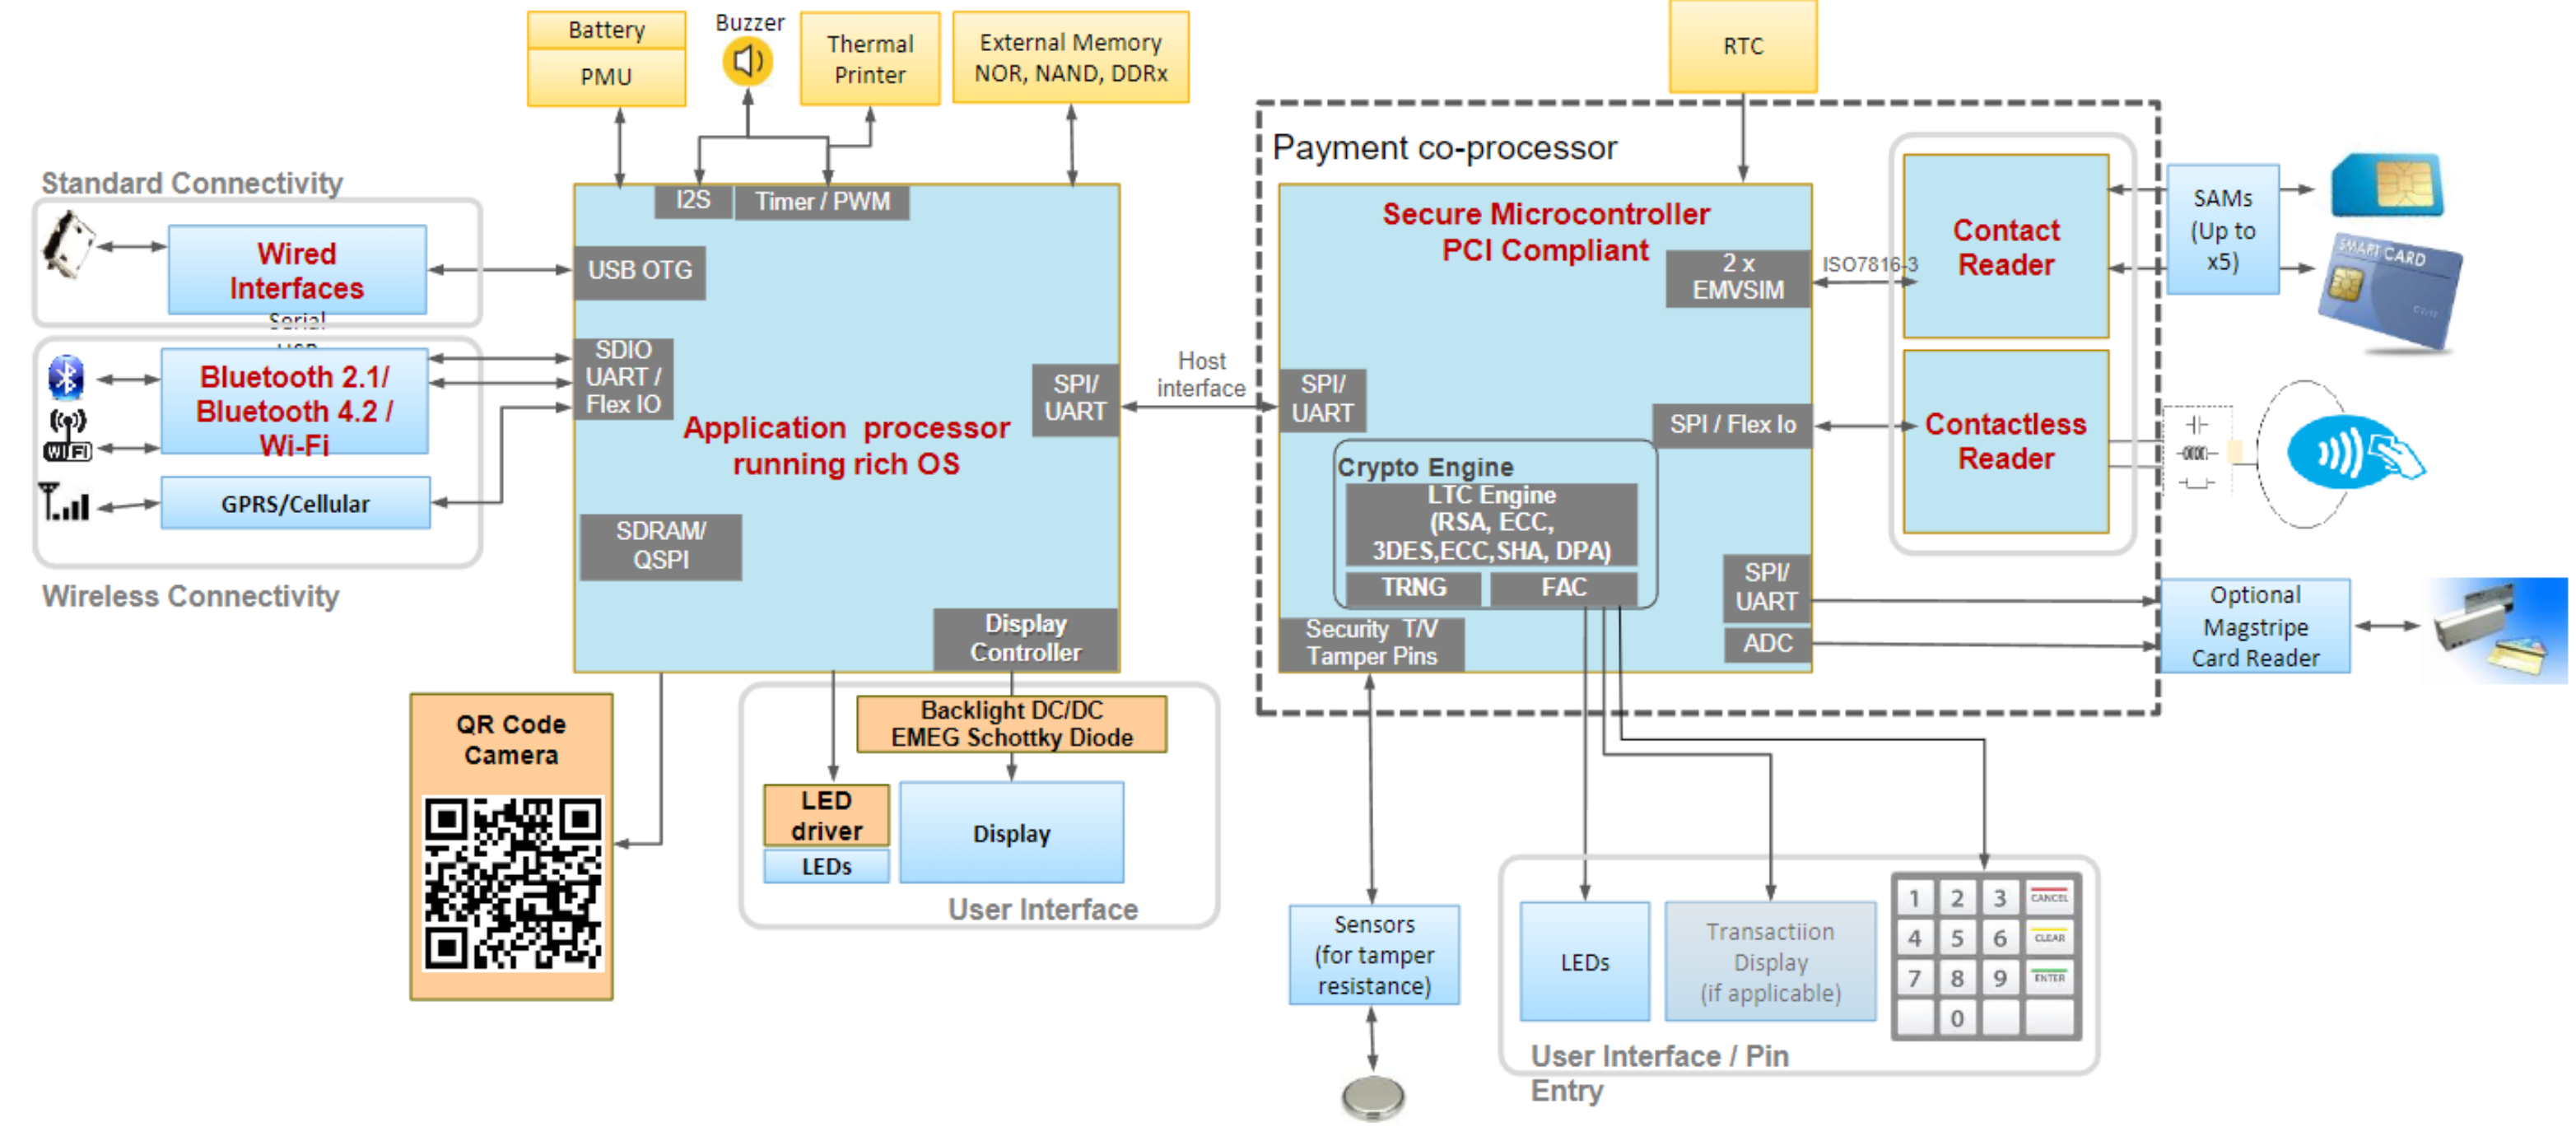
\includegraphics[width=1\textwidth]{images/research/postrem_struct}
    \caption{\centering Распространенная структура POS-терминала}
    \label{fig:postrem_struct}
\end{figure}

К обязательным элементам данного устройства можно отнести следующие:

\begin{itemize}
    \item RFID считыватель для обнаружения и связи со средствами платежа бесконтактным образом;
    \item модули проводной и/или беспроводной связи для связи с устройством-хостом или прямой связи с банком-эквайером.
\end{itemize}

Стоит отметить, что работа подобного устройства не возможна без программного обеспечения, интегрированного в POS-систему, которое управляет формированием и обработкой транзакций, шифрованием данных, запросами на авторизацию и связь с платежными сетями.

Одной из разновидностей торгового эквайринга является мобильный эквайринг, в нем в качестве платежного терминала используется mPOS- и softPOS-терминалы.

\begin{itemize}
    \item mPOS-терминал~--- это портативное устройство, состоящее из смартфона или планшета с подключенным внешним аппаратным модулем для работы с банковскими картами, которое используется для приема платежей;
    \item softPOS терминал~--- это программное решение, с помощью которого мобильное устройство с поддержкой NFC (как правило смартфон или планшет) выступает в роли платежного терминала, т.е. принимает бесконтактные средства платежа, используя встроенный модуль NFC, и осуществляет прием платежей~\cite{pos_term}.
\end{itemize}

Детальное сравнение разновидностей POS-терминалов приведено в таблице~\ref{tab:pos_comparison}.
\begin{longtable}[l]{|
P{0.2\textwidth}|
P{0.23\textwidth}|
P{0.23\textwidth}|
P{0.24\textwidth}|}

    \caption{Сравнение POS, mPOS и SoftPOS терминалов}
    \label{tab:pos_comparison} \\
    \hline
    \textbf{Особенность} &
    \textbf{POS-терминалы} &
    \textbf{mPOS-терминалы} &
    \textbf{SoftPOS-терминалы} \\
    \hline
    \endfirsthead

    \caption*{Продолжение таблицы~\ref{tab:pos_comparison}} \\
    \hline
    \textbf{Особенность} &
    \textbf{POS-терминалы} &
    \textbf{mPOS-терминалы} &
    \textbf{SoftPOS-терминалы} \\
    \hline
    \endhead

    \endfoot

    \endlastfoot

    Требования к оборудованию &
    специальные аппаратные компоненты &
    мобильное устройство с выходом в сеть и Bluetooth и внешний считыватель карт &
    смартфон или планшет с поддержкой NFC \\
    \hline

    Мобильность &
    стационарный &
    мобильный &
    мобильный \\
    \hline

    Методы оплаты &
    любые виды платежей &
    любые виды платежей &
    бесконтактные платежи \\
    \hline

    Особенности настройки &
    необходимость интеграции с сетью и окружением &
    требуется установка приложения на мобильное устройство с выходом в сеть и подключение считывателя карт &
    только установка приложения на устройство с выходом в сеть \\
    \hline

    Пользователь\-ский интерфейс &
    отдельный экран устройства &
    экран мобильного устройства и экран считывателя &
    экран мобильного устройства \\
    \hline
\end{longtable}


mPOS-терминалы занимают промежуточное положение между стационарными POS-устройствами и программными SoftPOS-решениями.
Их ключевое преимущество в высокой степени универсальности, сочетающей в себе мобильность и возможность работы с любыми типами карт — контактными, бесконтактными, а также с поддержкой магнитной полосы.

В отличие от стационарных POS-терминалов, которые требуют фиксированного места установки и имеют ограниченную мобильность, mPOS-устройства ориентированы на ТСП, чья деятельность связана с выездной торговлей, доставкой или оказанием услуг вне стационарных точек.
Это делает их особенно популярными среди малого бизнеса, самозанятых и индивидуальных предпринимателей, которым важно иметь возможность принимать оплату в любом месте без необходимости приобретения дорогостоящего оборудования.

SoftPOS-терминалы также обеспечивают высокую степень мобильности и минимальные затраты на оборудование, так как не требуют внешних считывателей.
Однако их применение ограничено устройствами с поддержкой NFC, а также повышенными требованиями к безопасности самого смартфона.
Такие терминалы пока не получили массового распространения в России, поскольку требуют глубокой интеграции с ОС и значительных усилий со стороны разработчиков для соответствия стандартам PCI PTS и EMV Level 2.

mPOS-терминалы работают на базе любого смартфона, поддерживающего Bluetooth или USB-подключение, совместимы с широким спектром банковских приложений и могут быть использованы даже со слабо защищёнными или устаревшими устройствах.
При этом уровень безопасности обеспечивается благодаря сертифицированному аппаратному модулю, через который проходит считывание данных с карты.

Продолжением развития мобильных терминалов можно считать смарт-терминалы~--- программно-аппаратные устройства состоящие из устройства на базе высокоуровневой ОС, например, Android и считывателя платежных карт.
Структура такая же как у mPOS-терминала, однако устройства находятся в едином корпусе и для их подключения, как правило, используется проводной метод.

Разработанный в рамках данной работы mPOS-терминал потенциально может быть адаптирован под формат смарт-терминала.
Такая конструкция обеспечивает не только удобство эксплуатации, но и возможность гибкой настройки интерфейса, расширения функциональности и интеграции с CRM- или ERP-системами.

Переход от mPOS к смарт-терминалу возможен, если:

\begin{enumerate}
    \item считыватель и смартфон будут объединены в единый корпус;
    \item устройство будет оснащено автономным питанием и возможностью выхода в интернет;
    \item будет реализована поддержка различных способов оплаты (QR-коды, HCE, токенизация).
\end{enumerate}

Это делает mPOS-терминал гибким решением, которое может развиваться в сторону более сложных и функциональных устройств, сохраняя при этом основные преимущества: низкую стоимость, простоту внедрения и высокую степень мобильности.


\subsubsection{Сравнение существующих устройств}

На российском рынке услугу мобильного эквайринга предлагаются различными банками, а также специализированные поставщики оборудования.
Банки преимущественно предоставляют услуги эквайринга с использованием стационарные POS-систем, они имеют высокую привязку к месту установки, поэтому их применение в мобильном бизнесе (бизнес, предусматривающий продажу товаров и оказание услуг на выезде) ограничено.
Сбербанк предоставляет услуги мобильного эквайринга на базе mPOS-терминалов фирмы Эвотор, которые выступают не только в качестве платежного устройства, но и в качестве фискального накопителя для осуществления учета товара~\cite{sber_acq}.

Специализированные поставщики оборудования, такие как 2can осуществляют производство mPOS-терминалов, ПО для них, а также разработку собственного softPOS-решения.
Они осуществляют партнерское взаимодействие с банками, предоставляя услуги эквайринга по фиксированной стоимости, и за фиксированный процент со всех успешно проведенных платежных операций~\cite{2can_mpos}.
А также реализуют совместимость терминала с платежными приложениями других компаний, например <<1C: Мобильная касса>> посредством разработки и поддержки интеграционного приложения, а также использования актуальных аппаратных решений (терминалов), сертифицированных регулирующими органами.

Сравнением технологических характеристик распространенных mpos-терминалов представлено в таблице~\ref{tab:mpos_comparison}.
% устройства первоначально были взяты с https://v8.1c.ru/1s-kassa/mobilnoe-prilozhenie-1s-mobilnaya-kassa/   `1С:Мобильную кассу на смартфоне`
\begin{longtable}[l]{|
P{0.15\textwidth}|
P{0.14\textwidth}|
P{0.14\textwidth}|
P{0.14\textwidth}|
P{0.14\textwidth}|
P{0.14\textwidth}|}

    \caption{Сравнение характеристик mPOS-терминалов}
    \label{tab:mpos_comparison} \\
    \hline
    \textbf{Характе\-ристика} &
    \textbf{PAX D230} &
    \textbf{Verifone VX675} &
    \textbf{Aisino VM30} &
    \textbf{Ingenico iPP320} &
    \textbf{2can P17} \\
    \hline
    \endfirsthead

    \caption*{Продолжение таблицы~\ref{tab:mpos_comparison}} \\
    \hline
    \textbf{Характе\-ристика} &
    \textbf{PAX D230} &
    \textbf{Verifone VX675} &
    \textbf{Aisino VM30} &
    \textbf{Ingenico iPP320} &
    \textbf{2can P17} \\
    \hline
    \endhead

    \endfoot

    \endlastfoot

    Поддержка Wi-Fi &
    да & нет & да & нет & нет \\
    \hline

    Поддержка GPRS/3G &
    да & да & да & нет & нет \\
    \hline

    Версия сертификата PCI PTS &
    6.x & 3.0 & 5.x & 3.x & 3.1 \\
    \hline

    Интеграция с платежным сервисом &
    зависит от банка & зависит от банка & зависит от банка & зависит от банка & SDK и REST API \\
    \hline

    Стоимость (мин.), тыс.\ рублей &
    23 & 11 & 9 & 19 & 8 \\
    \hline
\end{longtable}

% Verifone VX675 - https://techplat.ru/pos---terminal-verifone-vx-675-wi-fibtctls/  https://mirbeznala.ru/product/verifone-vx675-gprs-ctls-b-u/
% Aisino VM30 - https://cnvanstone.en.made-in-china.com/product/NJBrmIbTbFcD/China-Cheapest-Contactless-Card-Payment-Machine-Vm30-Mpos-Card-Reader.html  (цена)https://mirbeznala.ru/product/mpos-terminal-aisino-vm30/?srsltid=AfmBOorvKHSmqTDupSOvhsfPhqaJosEoSJpBhtb5Py6Hxlca2d3oy_uJ
% Ingenico iPP320 - https://mirbeznala.ru/product/ingenico-ipp-320-novyy/?srsltid=AfmBOooqXx7twi2Wg_25vM7lI9phsazEMrYhy-tb49VgRkWvph4EDY-m#char
% 2can P17 - https://1c.ru/news/info.jsp?id=23121

% убрал из сравнения: PAX D210E - https://mirbeznala.ru/product/perenosnoy-terminal-pax-d210e/

Все устройства подключаются к мобильному устройству по Bluetooth (версии различаются, но их различия оказывают незначительное влияние на работу) поддерживают бесконтактную оплату и сертифицированы по стандартам EMV L1\&L2 и EMV Contactless L1, посредством интеграции с внешним ПО поддерживают интеграцию с ОФД (операторами фискальных данных), т.е. системой учета товаров.

Сертификация EMV Level 1 подтверждает соответствие считывателя карты требованиям стандарта EMV по электрическим, механическим и функциональным параметрам.

Сертификация EMV Level 2 подтверждает соответствие программного обеспечения, реализующего обработку платежных транзакций стандарту EMV в части функциональных тестов по выполнению основных функций обработки транзакций;

PCI PTS (Payment Terminal Security)~--- это стандарт безопасности, разработанный PCI Security Standards Council, который устанавливает требования к защите аппаратных устройств, используемых для обработки данных карты (POS-терминалов, mPOS, ATM и т.д.).
Этот стандарт призван обеспечить высокий уровень защиты от несанкционированного доступа к конфиденциальной информации: данным магнитной полосы, номеру карты, PIN-коду, ключам шифрования и другим данным.

% TODO: можно добавить про классификацию с сайта
%  https://mst-company.ru/blog/ekvajring-tipy-pos-terminalov-klassifikatsiya-emvco-i-platezhnykh-sistem

\subsection{Стандарт платежных карт EMV}

В подразделе~\ref{subsec:payment_process} были рассмотрены стандартные сценарии выполнения платежных операций.
В рамках разработки системы отдельного внимания заслуживают процессы взаимодействия платежного терминала с банковской картой (или мобильным платежным приложением) и с хостом банка-эквайера.
Анализа данных процессов и используемых в них технологий позволит обеспечить корректность работы разрабатываемой системы.

Наиболее важным в данном контексте является стандарт EMV, т.к. он описывает характеристики банковских карт и других средств оплаты, а также весь процесс формирования платежа.
ФСБ РФ совместно с ЦБ РФ определяют классификацию платежных устройств и устанавливают для них ряд функциональных требований на основе стандарта EMV~\cite{cbr_requirements}.

Требования к считывателю смарт-карт и протоколу взаимодействия с ними описаны в 4 книгах <<EMV Integrated Circuit Card Specifications for Payment Systems>>, которые затрагивают следующие аспекты:
\begin{itemize}
    \item книга 1 описывает требования интерфейса платежного терминала для взаимодействия со смарт-картой независимо от используемого платежного приложения;
    \item книга 2 описывает аспекты безопасности и хранения ключей доступа на платежных картах и терминалах для обеспечения их корректной работы и взаимодействия, а также дополнительные требования и рекомендации в отношении онлайн-связи между картой и эмитентом, управления
    криптографическими ключами на уровне терминала, эмитента и платежной системы.;
    \item книга 3 определяет процедуры взаимодействия терминала и платежной карты, необходимые для осуществления транзакции платежной системы;
    \item книга 4 определяет обязательные, рекомендуемые и необязательные требования к терминалу, необходимые для поддержки приема карт.
\end{itemize}

Требования для считывателя бесконтактных карт определены в <<EMV Level 1 Specifications for Payment Systems, EMV Contactless Interface Specification>>, а требования к протоколу обмена между считывателем и бесконтактной картой описаны в книгах <<EMV Contactless Specifications for Payment Systems>>:
\begin{itemize}
    \item книга A описывает архитектуру POS-терминала бесконтактной оплаты и общие требования к нему;
    \item книга B определяет спецификацию работы Entry Point~--- ПО, отвечающего за взаимодействие терминала и бесконтактной картой: выбор платежного приложения, активацию платежного ядра и использование его результатов;
    \item книги C (2-8) содержат описание принципов работы платежных ядер различных ПС.
\end{itemize}

Также для бесконтактных карт есть книга E, которая выступает в качестве аналога книге 2 из серии <<EMV Integrated Circuit Card Specifications for Payment Systems>>, также фокусируюсь на вопросах безопасности и хранения и использования ключей доступа, но уже на бесконтактных платежных картах.



EMV~--- стандарт для банковских карт, совместно разработанный платежными системами Europay, Mastercard и Visa.
Он используется  международными платежными системами (МПС) для проведения операций по банковским картам.

Повышенный уровень безопасности карт стандарта EMV обусловлен наличием встроенного чипа, который называется Secure Element.
Чип хранит данные в зашифрованном формате, а также может запускать приложения на карте и обмениваться командами с кассовыми терминалами.

Банковская карта с поддержкой стандарта EMV, является стандартной смарт-картой, однако, имеет расширенный функционал.
Технология функционирования платежной карты (как контактной, так и бесконтактной) и взаимодействия платежного терминала с ней описана в стандарте ISO/IEC 7816 и в <<EMV Integrated Circuit Card Specifications for Payment Systems>>.
Технология работы с бесконтактной картой описана в стандарте ISO/IEC 14443, а также в <<EMV Contactless Specifications for Payment Systems>>.
Карта имеет операционную систему со встроенной файловой системой и приложениями, причем предназначенными не только для реализации платежей~\cite{emv_specifications_book}.

\subsubsection{EMV-карта}

Главное новшество EMV-карт~--- возможность проверки динамической криптограммы карты (цифровой подписи ее статических данных).
Для карт с магнитной полосой терминалы не имели такую возможность и выполняли проверку только статических данных карты, в результате чего такие карты легко копировались.
Процесс аутентификации карты с магнитной полосой и EMV-карты представлен на рисунках~\ref{fig:magnetic_card_auth} и~\ref{fig:emv_card_auth} соответственно.

\begin{figure}[H]
    \centering
    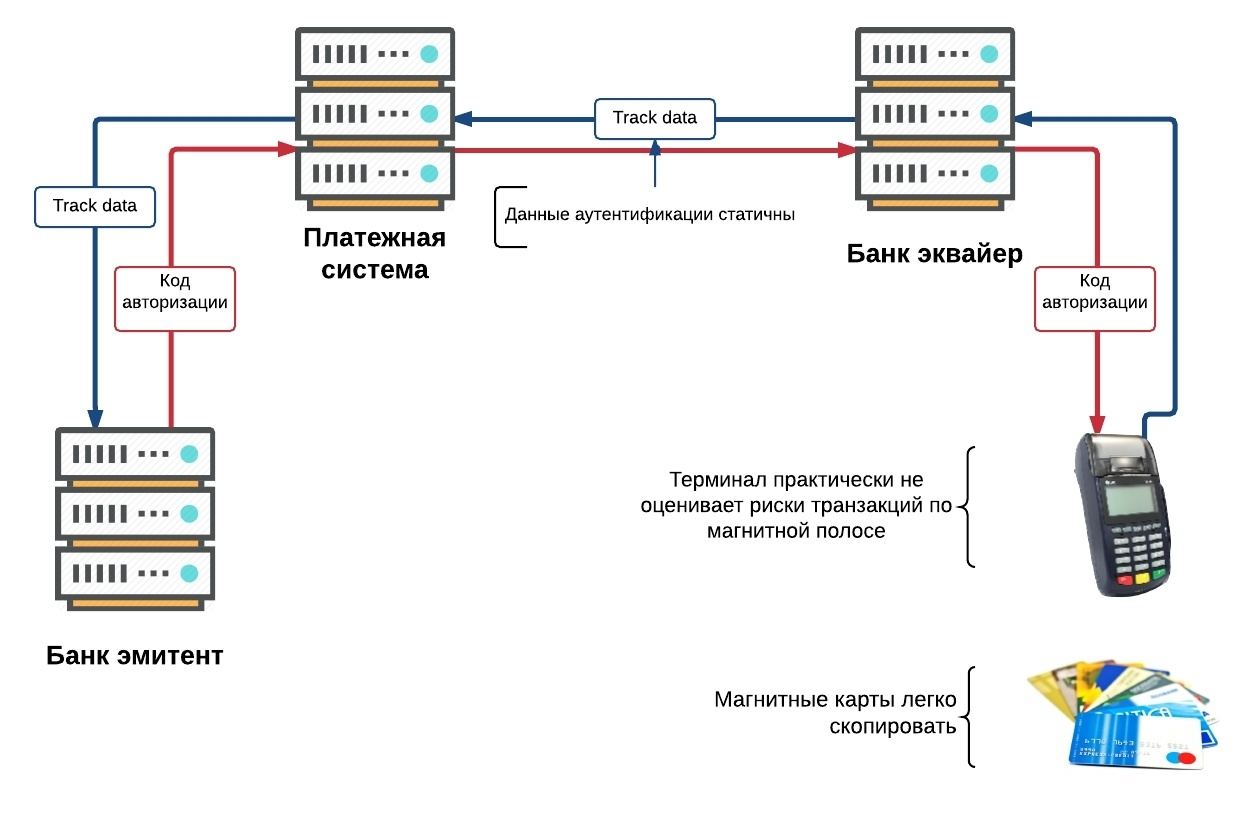
\includegraphics[width=0.8\textwidth]{images/research/magnetic_card_auth}
    \caption{\centering Аутентификации карты с магнитной полосой в ходе платежной транзакции}
    \label{fig:magnetic_card_auth}
\end{figure}

\begin{figure}[H]
    \centering
    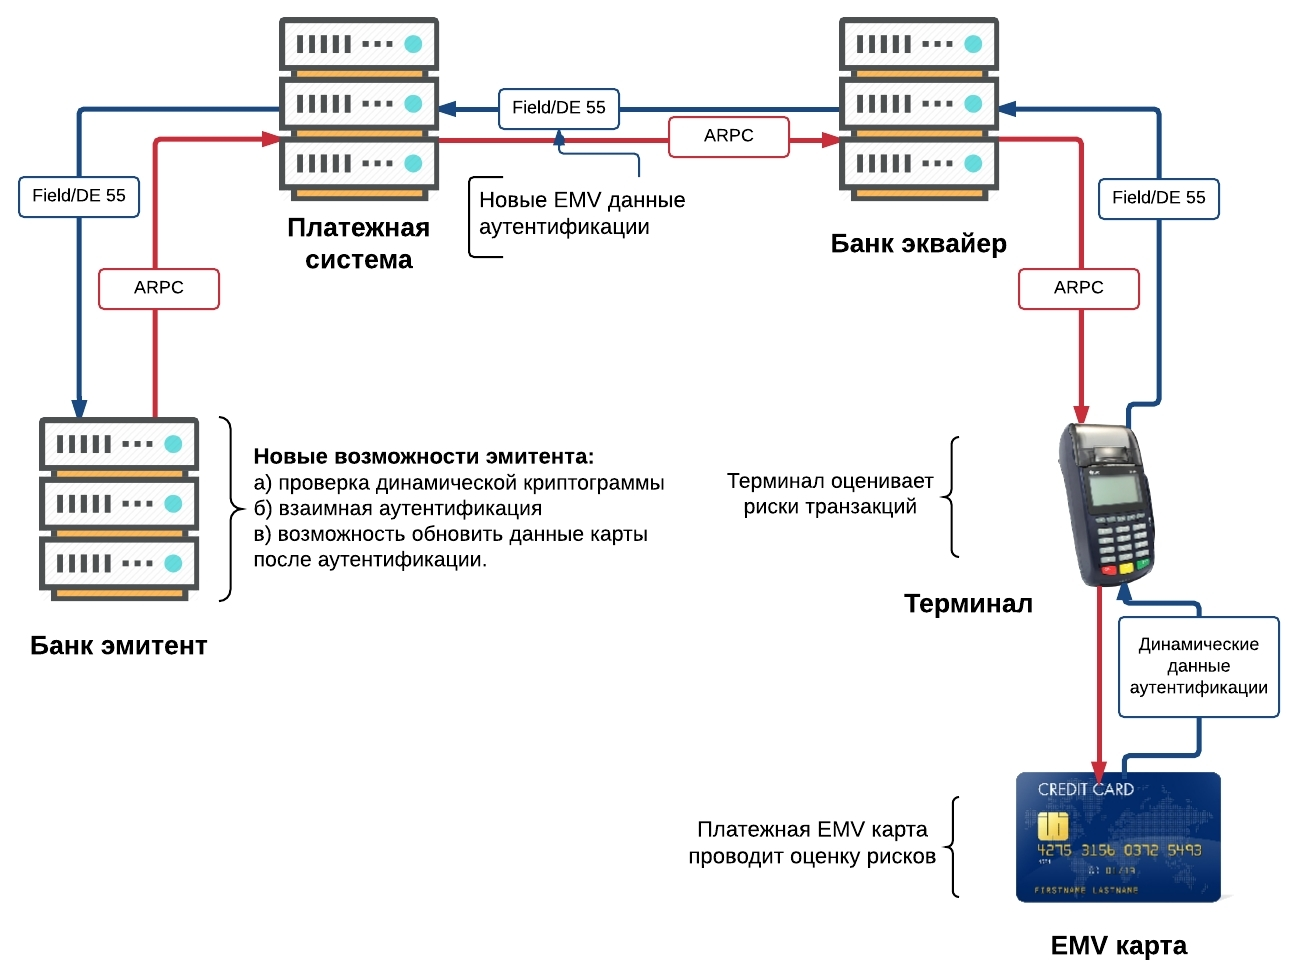
\includegraphics[width=0.8\textwidth]{images/research/emv_card_auth}
    \caption{\centering Аутентификации EMV-карты на основе динамической криптограммы в ходе платежной транзакции}
    \label{fig:emv_card_auth}
\end{figure}

Динамическая аутентификация карты в ходе EMV-транзакции происходит по следующему алгоритму:

\begin{enumerate}
    \item терминал передает данных о транзакции на карту (сумма, валюта, страна и пр.);
    \item происходит проверки рисков транзакции как картой, так и терминалом;
    \item если проверка не пройдена на карте, то процесс прерывается, если пройдена~-- карта подписывает данные транзакции;
    \item терминал помечает полученными от карты данные тегом <<DE 55>> (стандарт ISO 8583) и отправляет вместе с прочими в банк-эквайер;
    \item банк-эмитент выполняет проверку динамической подписи транзакции.
\end{enumerate}

Данные в Field/DE 55 содержится важная информация для оценки рисков транзакции  эмитентом и ПС, в частности Terminal Verification Result и Card Verification Result~\cite{emv_card_mechanism}.

Банк-эмитент также может выслать свою криптограмму карте для дополнительной аутентификации или обновить данные карты (например, лимит карты), записанные на чипе карты (уже после успешной аутентификации)~\cite{emv_book_2}.
Более подробно процесс формирования и проверки криптограммы уже был описан в пункте~\ref{subsubsec:contactless_payment}.

\subsubsection{Платежные EMV-приложения}

Платежное EMV-приложение выступает в качестве интерфейса для взаимодействия с картой.
С помощью серии команд, поданных в приложение на карте осуществляется управление приложением и состоянием транзакции.

Для работы с приложениями на карте используются APDU-команды, описанные в стандарте ISO/IEC 7816--4, рассматриваемым в пункте~\ref{subsec:7816}.
С их помощью реализуется функционал приложения, например, создание банковской транзакции и управление ее состоянием.
Стоит также отметить, что производители карты реализуют свои собственные приложения для оплаты, реализуя при этом стандарт выполнения платежа в EMV, который называется EMV Transaction Flow, о нем речь пойдет в подпункте~\ref{subsubsec:emv_transaction}.

Каждое приложение имеет свой собственный идентификатор~--- AID (Application Identifier).
Он указывает к какому типу ПС относится приложение и для каких карт может использоваться (для карт одной ПС, могут использоваться разные приложения).
На основе идентификатора приложения AID терминал определяет возможность проведения транзакции или, в случае нескольких приложений, составляет список поддерживаемых приложений и предлагает выбрать одно из них для выполнение транзакции~\cite{emv_card_mechanism}.

\subsubsection{Безопасность EMV-карты}

Любые смарт-карты, и EMV-карты не исключение, имеют механизм разграничения доступа, с помощью которого происходит контроль состояния карты в рамках текущей сессии подключения и механизм проверки условий доступа, другими словами, проверка прав на работу с файлами.
Наличие прав зависит от состояния карты в рамках текущей сессии, которое может изменяться вводом определенных предварительно заложенных кодов доступа~\cite{habr_smart_card_for_little}.

Также смарт-карты имеют встроенные механизмы для шифрования, однако их аппаратная реализация отличается в зависимости от производителя.
В EMV-чипах реализованы следующие алгоритмы шифрования:

\begin{itemize}
    \item RSA (асимметричное шифрование): применяется в EMV-картах для аутентификации и защиты данных, используется для динамической аутентификации (DDA) и комбинированной аутентификации (CDA), обеспечивая высокий уровень безопасности за счет генерации уникальных ключей для каждой транзакции;
    \item DES и 3DES (симметричное шифрование): DES - устаревший и менее безопасный стандарт, однако по-прежнему применяемый в некоторых системах, более распространенным является 3DES (Triple DES), который обеспечивает улучшенную безопасность за счет применения алгоритма DES трижды, эти алгоритмы используются для шифрования PIN-кодов;
    \item AES (Advanced Encryption Standard): современный симметричный алгоритм шифрования, предлагающий более высокий уровень безопасности по сравнению с DES и 3DES, благодаря более длинным ключам и более сложным методам шифрования, используется в технологии HCE (Host Card Emulation) для шифрования в приложениях <<Цифровых кошельках>> на мобильных устройствах;
    \item SHA-1 и SHA-256 (хэширование): используется для создания хэш-значений транзакций, из-за уязвимостей SHA-1 многие системы переходят на SHA-256, который обеспечивает более высокий уровень безопасности, с помощью хэш-функции гарантируется целостность данных в процессе транзакций.
    % информация взята с "https://fastercapital.com/ru/content/%D0%A2%D0%B5%D1%85%D0%BD%D0%BE%D0%BB%D0%BE%D0%B3%D0%B8%D1%8F-%D1%87%D0%B8%D0%BF%D0%BE%D0%B2-EMV--%D0%B1%D0%B5%D0%B7%D0%BE%D0%BF%D0%B0%D1%81%D0%BD%D1%8B%D0%B5-%D0%B8-%D1%83%D0%BC%D0%BD%D1%8B%D0%B5--%D0%BA%D0%B0%D1%80%D1%82%D1%8B-Visa-%D0%B8-%D1%82%D0%B5%D1%85%D0%BD%D0%BE%D0%BB%D0%BE%D0%B3%D0%B8%D1%8F-EMV-Chip.html
\end{itemize}

Важно понимать, что персональная информация владельца карты в платежных приложениях не хранится, а сами приложения, ключи и некоторые PIN-коды, защищены от прямого доступа и модификации.
Однако, информация, не относящаяся к конфиденциальным данным, является доступной.
К подобной информации относятся различные данные, необходимые для выполнения платежных операций, в частности сертификаты ключей-доступа, номер карты (PAN), списки методов проверки карты (CVM~-- Card Verification Methods list) и другая информация.
Примерный перечень всех доступных для чтения данных приложения приведен на рисунке~\ref{fig:emv_available_data}.
Доступные данные организованы в записи (рекорды или треки), которые можно получить с помощью команд «Get Processing Options» и «Read Record», описанных  в ISO/IEC 7816.
Дополнительно данные технических настроек, таких как лимиты и счетчики, могут быть доступны через команду «Get Data» с указанием требуемого типа~\cite{emv_card_mechanism}.

\begin{figure}[H]
    \centering
    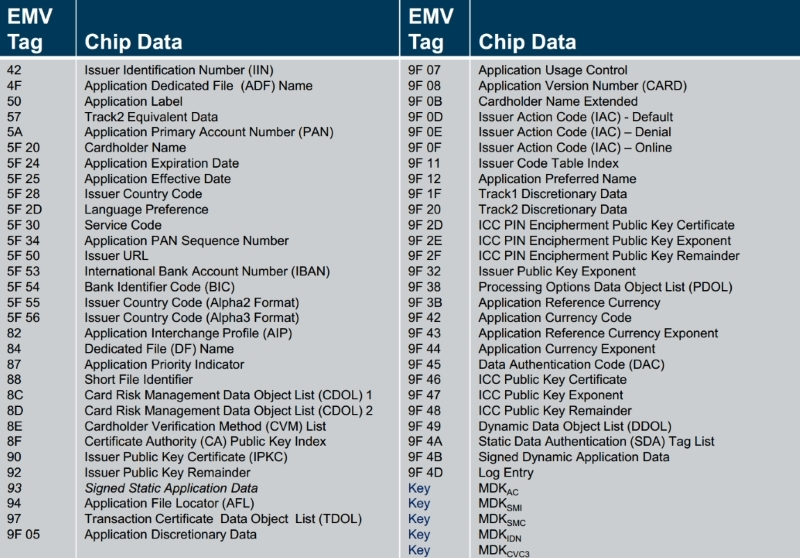
\includegraphics[width=0.8\textwidth]{images/research/emv_available_data}
    \caption{\centering Доступные данные платежного EMV-приложения}
    \label{fig:emv_available_data}
\end{figure}

Банковская платежная карта имеет несколько уровней защиты, определенных хронологией ее создания:

\begin{enumerate}
    \item производитель чипа карты задает некий первичный ключ для доступа к прошивке карты, с помощью него можно установить ОС;
    \item ОС карты также имеет свой ключ, который необходим для работы с файлами и приложениями на карте, с помощью него можно установить платежные приложения;
    \item платежные приложения на карте персонализируются с помощью определенных параметров и ключей приложения, заложенных банком-эмитентом с целью обеспечения безопасности EMV-транзакций.
\end{enumerate}

После чего, как правило, изменение работы карты и приложения становится практически невозможным без знания ключей.
Данные платежного приложения могут модифицироваться после выпуска карты посредством банкомата или терминала, которые после успешной аутентификации карты в ходе банковской транзакции, передает скриптовую командой, имеющую цифровую MAC-подписью, гарантирующей целостность данных.
Такая возможность предусмотрена для того, чтобы  банк-эмитент управлять блокировкой карты, обновлять лимиты или настройки.
В данном случае, MAC (Message Authentication Code)~--- это аналог цифровой подписи, который гарантирует целостность данных, переданных на карту.
Для его расчета используется соответствующий ключ приложения (один из 3-х DES ключей загружаемых в приложение).

Технически возможно перенести данные с одной банковской карты на другую, если приложение на новой карте не персонализировано.
Однако отсутствие возможности доступа, а, как следствие, и копирования ключей делает карту неприменимой для проведения транзакций, т.к. без них приложение не сможет сгенерировать корректную подпись транзакции, что приведет к отклонению операции банком-эмитентом.
Кроме того, невозможность выполнить CDA (Combined Data Authentication) или DDA (Dynamic Data Authentication) существенно ограничивает использование копии.
Единственным уязвимым местом может быть SDA (Static Data Authentication), однако этот метод уже считается устаревшим и редко используется как единственный механизм аутентификации~\cite{emv_card_mechanism}.

\subsubsection{EMV-транзакция}
\label{subsubsec:emv_transaction}

В пункте~\ref{subsubsec:contactless_payment} уже упоминалось о существовании 2-х типов платежный транзакций: онлайн и офлайн, а также в общих чертах было рассмотрено выполнение онлайн транзакции.
Есть также 2 способа аутентификации: офлайн или Static Data Authentication (SDA) и онлайн или Dynamic Data Authentication (DDA).
Онлайн аутентификация проводится при непосредственном участии эмитента.
Офлайн-аутентификация, в свою очередь, выполняется самим платежным терминалом.
Важно отметить, что при обработке онлайн-операции могут одновременно использоваться как онлайн, так и офлайн аутентификация, если карта и терминал поддерживают оба метода, такой вид аутентификации называется Combined Data Authentication (CDA).

Любая платежная транзакция в соответствии со стандартом EMV начинается с выбора платежного приложения на терминале.
После выбора приложения терминал и карта выполняют ряд функций, которые схематично представлены на рисунке~\ref{fig:transaction_flow_example} в порядке своего выполнения.
Для каждой функции есть условия и ограничения применения, которые детально описываются стандартом.
В соответствии с EMV стандартом терминал во время транзакции должен выполнять только те функции, которые поддерживаются конкретной платежной картой~\cite{emv_book_3}.


\begin{figure}[H]
    \centering
    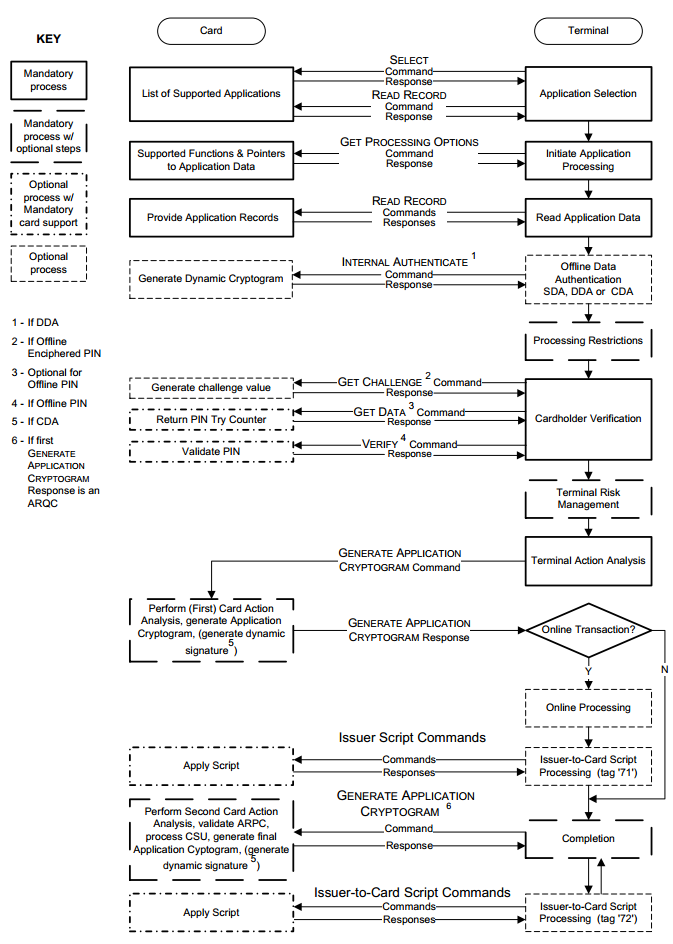
\includegraphics[width=0.8\textwidth]{images/research/transaction_flow_example}
    \caption{\centering Схема алгоритма выполнения транзакции терминалом}
    \label{fig:transaction_flow_example}
\end{figure}

За безопасность проведения транзакции отвечают следующие этапы:

\begin{itemize}
    \item аутентификация (офлайн, онлайн или комбинированная);
    \item оценка рисков проведения транзакции;
    \item верификация держателя карты на основе онлайн и/или офлайн PIN-кода, размера суммы транзакции, страны, валюты и прочих данных;
\end{itemize}

Процесс выполнения онлайн аутентификации представлен на рисунке~\ref{fig:online_auth}.
Его описание было приведено в пункте~\ref{subsubsec:contactless_payment}.

\begin{figure}[H]
    \centering
    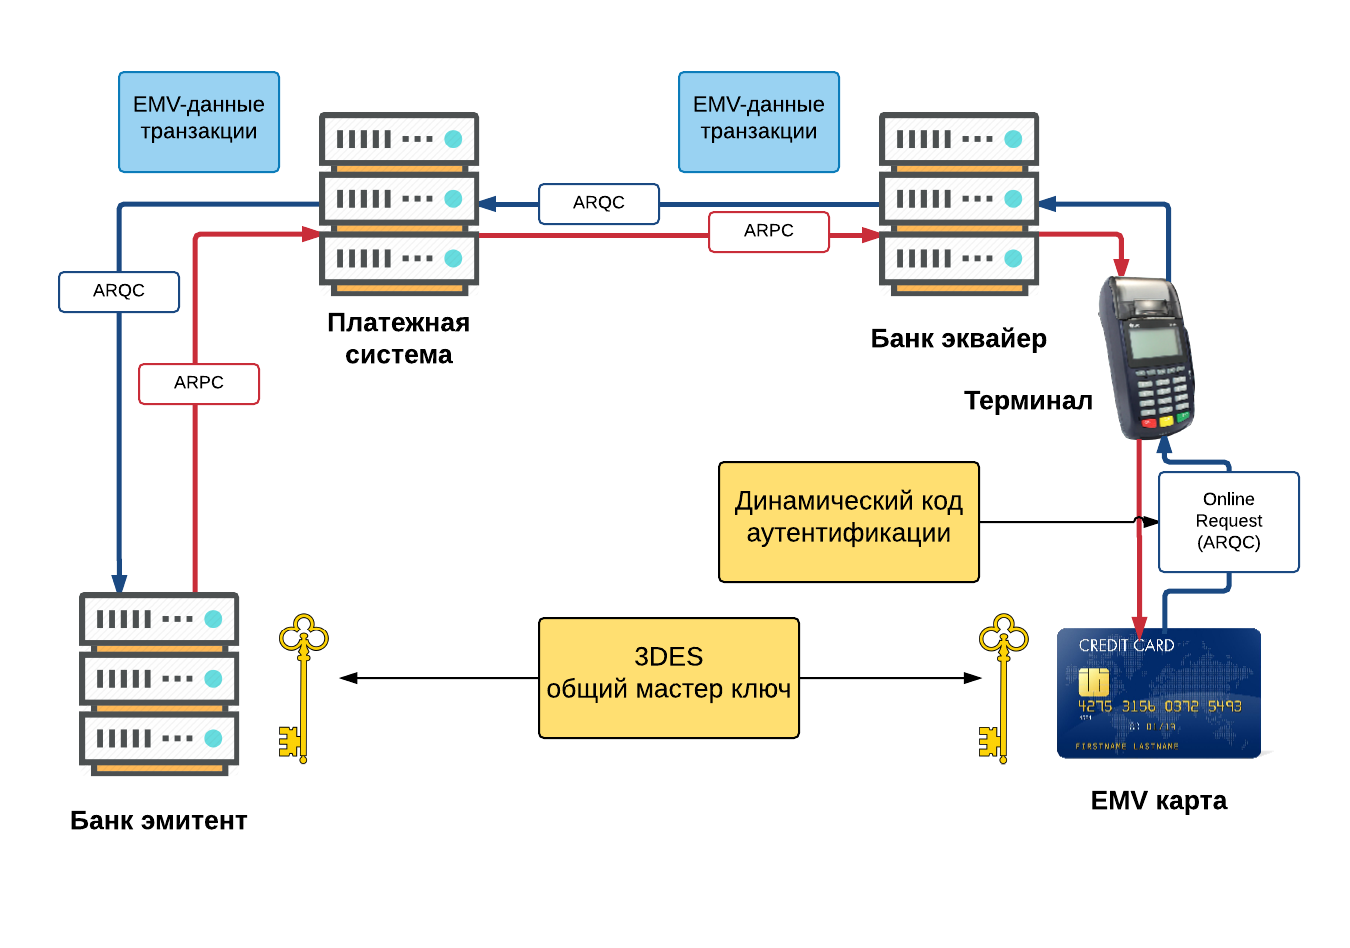
\includegraphics[width=0.8\textwidth]{images/research/online_auth}
    \caption{\centering Процесс выполнения онлайн аутентификации}
    \label{fig:online_auth}
\end{figure}


Офлайн аутентификация, как уже отмечалось ранее, происходит без непосредственного взаимодействия с банком или ПС в момент совершения операции.
Карта и терминал могут самостоятельно одобрить транзакцию, если её сумма не превышает установленный лимит.
Терминал же передает информацию в банк в соответствии с установленным режимом.
Преимущества данного подхода в том, что держатель карты может завершить оплату при отсутствии связи с банком, и операции на небольшие суммы выполняются значительно быстрее.

Офлайн аутентификация происходит с использованием асимметричной криптографии RSA.
Основная причина использования RSA заключается в распределении ключей: в онлайн-транзакциях ключи известны только карте и банку, тогда как в офлайн-процессе терминал также должен иметь доступ к ключу.
С учетом большого количества терминалов, повышается вероятность компрометации секретного ключа, что делает асимметричный подход более безопасным, т.к. терминал хранит только открытый ключ, а карта - секретный ключ.

Упрощенная модель статической аутентификации (Static Data Authentication) представлена на рисунке~\ref{fig:sda}.

\begin{figure}[H]
    \centering
    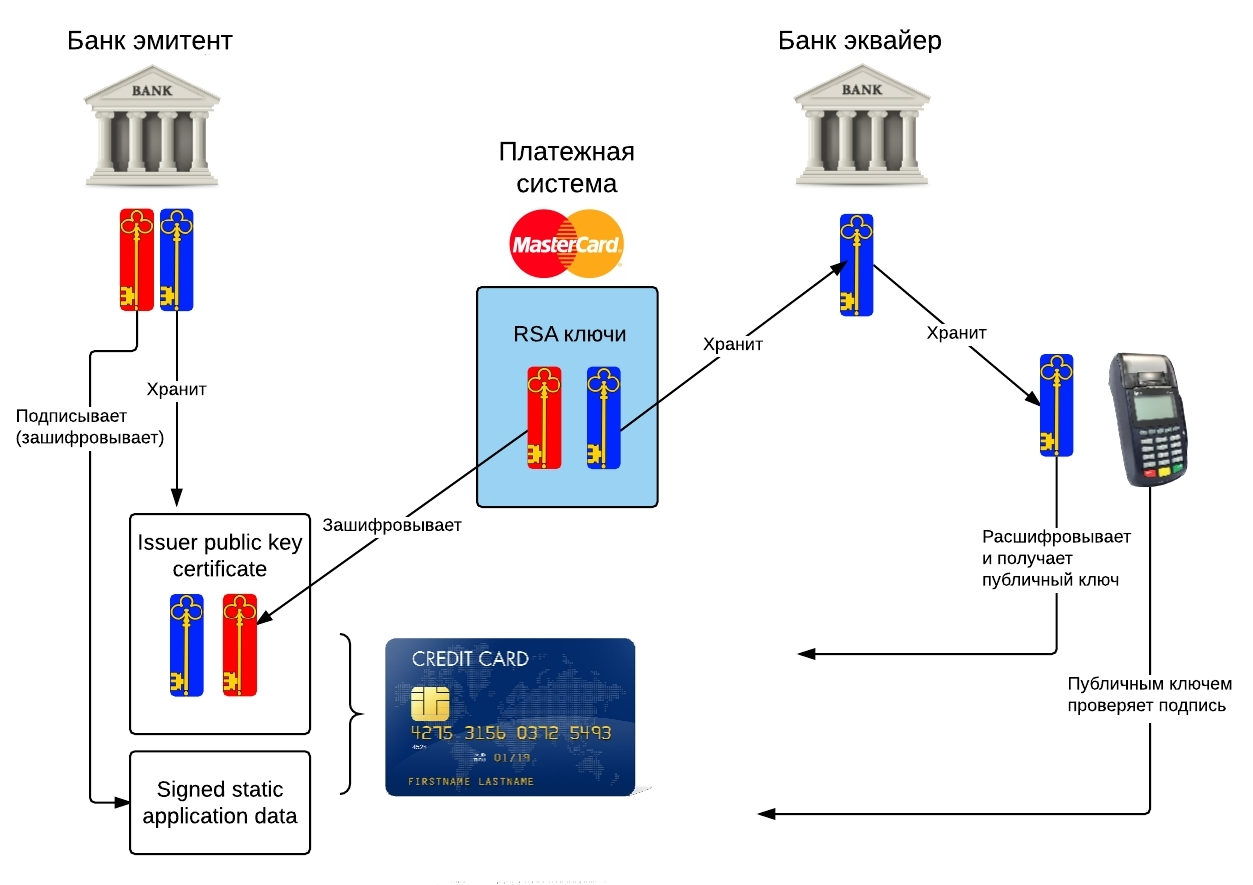
\includegraphics[width=0.8\textwidth]{images/research/sda}
    \caption{\centering Упрощенная модель Static Data Authentication (SDA)}
    \label{fig:sda}
\end{figure}

Центральную роль в этом процессе играет ПС, выступающая в качестве сертификационного центра, она создает пару ключей: секретный (красный) и открытый (синий).
Аналогичную пару ключей генерирует банк-эмитент.
Публичный ключ эмитента включается в специальный сертификат (Issuer Public Key Certificate), подписанный с использованием приватного ключа ПС.
Данный сертификат загружается на карту в процессе ее персонализации.

Когда платежный терминал подключается к торговой точке, в него загружается публичный ключ ПС через банк-эквайер.

Во время выполнения офлайн транзакции терминал осуществляет аутентификацию карты по следующему алгоритму:

\begin{enumerate}
    \item терминал считывает сертификат банка-эмитента (Issuer Public Key Certificate) с карты и с помощью публичного ключа ПС проверяет его подпись;
    \item если подпись сертификата подтверждена, терминал извлекает публичный ключ банка-эмитента из сертификата;
    \item данный ключ используется для проверки подписи критически важных данных карты, что позволяет удостовериться в её подлинности.
\end{enumerate}


% TODO: можно удалить абзац и картинку, если будет превышение объема
Описание выполнение SDA из стандарта EMV приведено на рисунке~\ref{fig:emv_offline_sda}~\cite{emv_book_2}.

\begin{figure}[H]
    \centering
    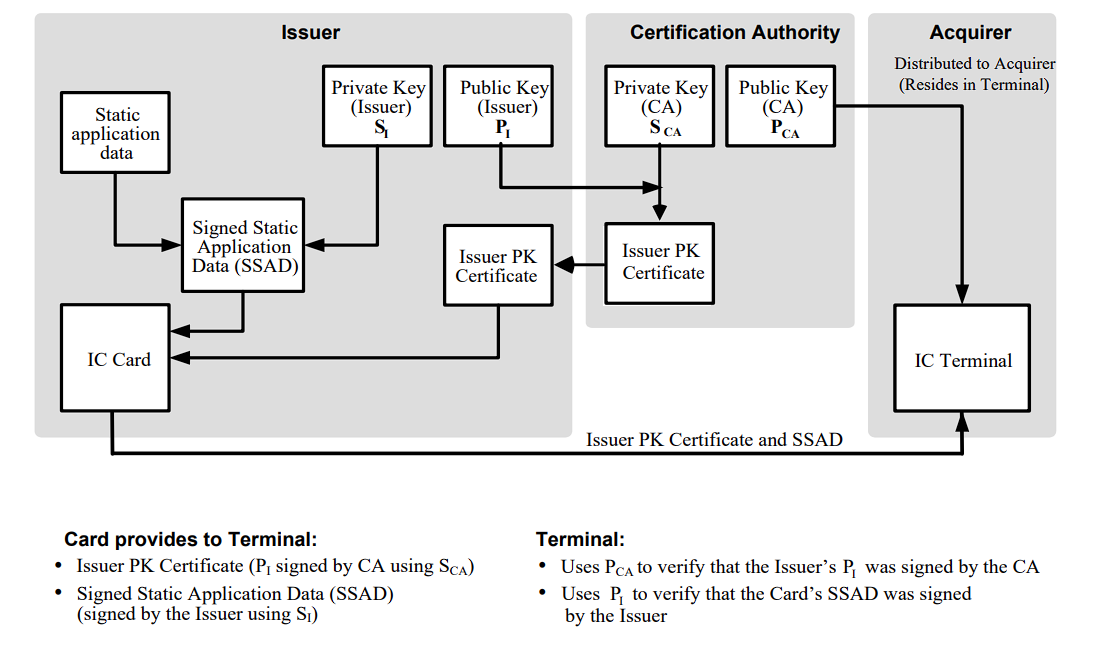
\includegraphics[width=0.8\textwidth]{images/research/emv_offline_sda}
    \caption{\centering Диаграмма Static Data Authentication (SDA)}
    \label{fig:emv_offline_sda}
\end{figure}

SDA в настоящее время уступает место более современным технологиям DDA (Dynamic Data Authentication) и CDA (Combined Data Authentication).
Эти методы включают в себя SDA, но также используют динамическое подписание данных, передаваемых между терминалом и картой.

Технология SDA позволяет удостовериться в неизменности данных на карте, но не обеспечивает полной защиты от копирования.
В отличие от неё, DDA и CDA подтверждают подлинность карты, поскольку карта хранит уникальный приватный ключ.
Сертификат этого ключа подписан приватным ключом эмитента, а сертификат эмитента~-- приватным ключом платежной системы.

DDA и CDA схожи по структуре: оба используют уникальный ключ карты и динамические данные.
Однако DDA выполняется как отдельная операция до начала основной транзакции, тогда как CDA интегрирована в транзакционный процесс и дополнительно подписывает криптограмму карты.
Несмотря на то, что CDA обеспечивает более высокий уровень безопасности, на практике чаще применяется DDA.

Описание выполнение офлайн DDA и CDA из стандарта EMV приведено на рисунке~\ref{fig:emv_offline_dda_cda}~\cite{emv_book_2}.

\begin{figure}[H]
    \centering
    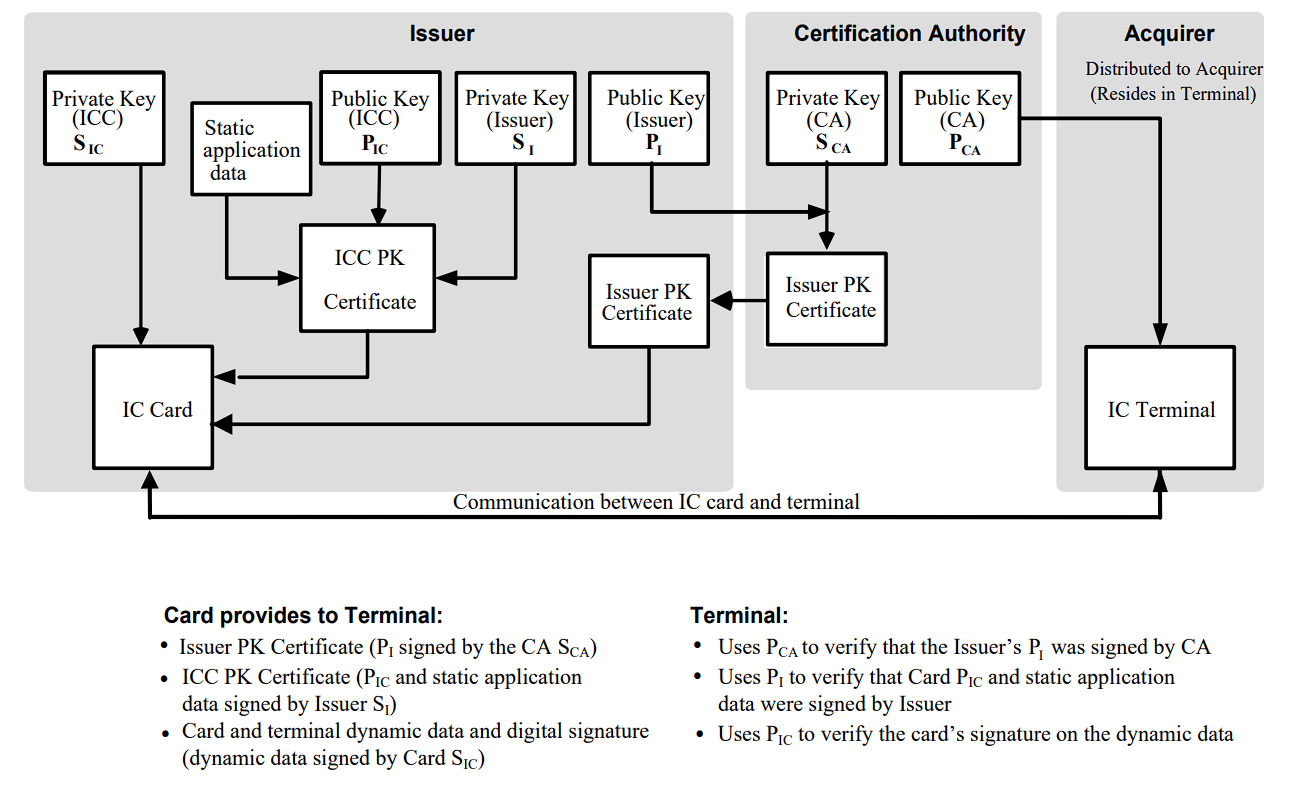
\includegraphics[width=0.8\textwidth]{images/research/emv_offline_dda_cda}
    \caption{\centering Диаграмма офлайн DDA и CDA}
    \label{fig:emv_offline_dda_cda}
\end{figure}

Также существует алгоритм офлайн DDA с использованием криптографии эллиптических кривых (Elliptic Curve Cryptography~-- ECC), который называется
Extended Data Authentication (XDA).

Описание выполнение офлайн XDA стандарта EMV приведено на рисунке~\ref{fig:emv_offline_xda}~\cite{emv_book_2}.

\begin{figure}[H]
    \centering
    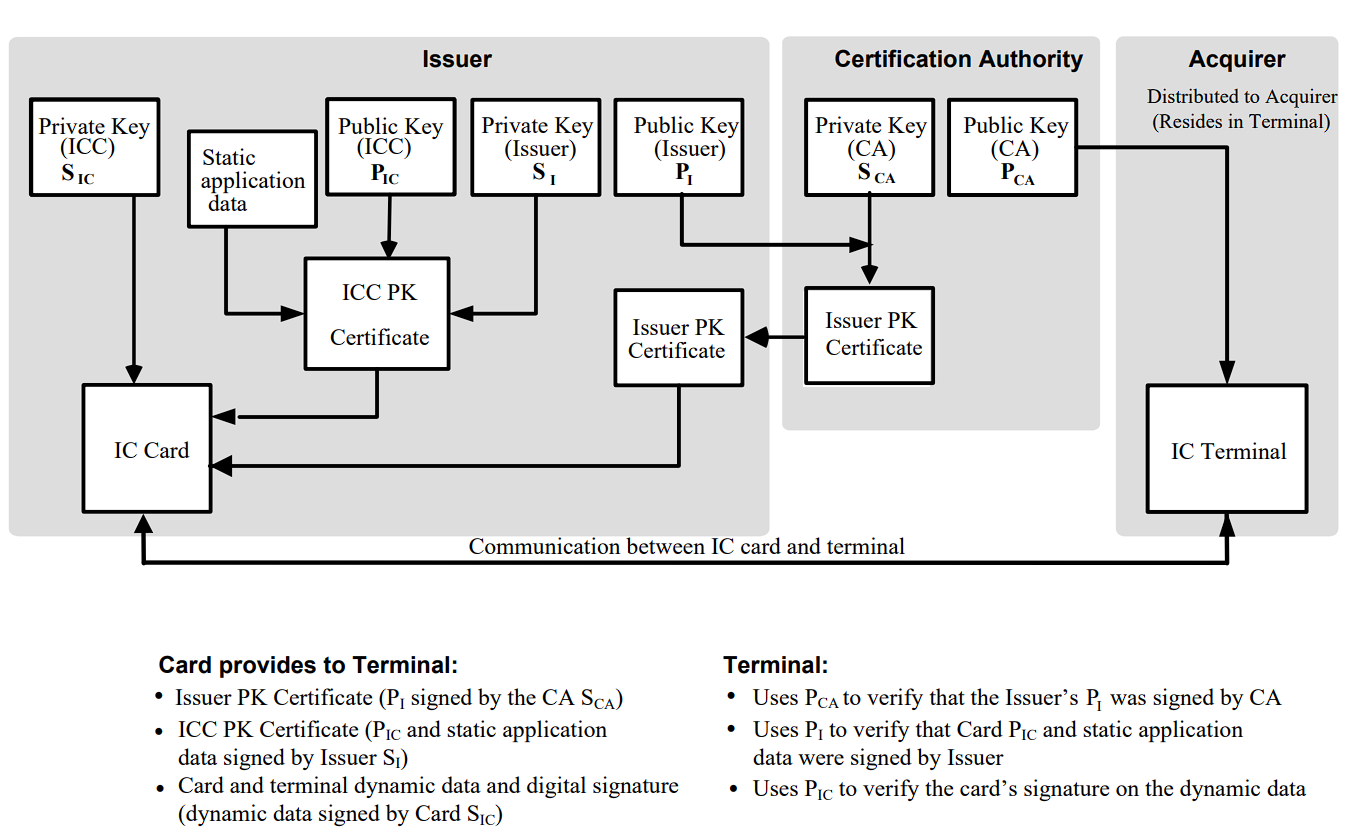
\includegraphics[width=0.8\textwidth]{images/research/emv_offline_xda}
    \caption{\centering Диаграмма офлайн XDA}
    \label{fig:emv_offline_xda}
\end{figure}


При выполнении XDA карта генерирует цифровую подпись, которая проверяется терминалом.
Эта подпись аутентифицирует карту и подтверждает подлинность кода аутентификации приложения (Application Cryptogram, AC), а также других критически важных данных, переданных картой и терминалом.
Это делает невозможным создание поддельной карты и обеспечивает целостность данных между картой и терминалом.

Для реализации XDA необходимо наличие центрального удостоверяющего центра (Certification Authority)~--- высоко защищённого криптографического устройства, которое подписывает открытые ключи эмитента.
Если приложение терминала поддерживает XDA, то оно должно содержать соответствующие открытые ключи удостоверяющего центра для данного приложения.

\subsubsection{Проверки безопасности транзакции}
\label{subsubsec:transaction_security_check}

Карты и терминалы также оценивают риски транзакций.
Для офлайн транзакций карта использует счетчики операций, лимиты сумм, правила проверки PIN-кода, а также другие параметры.
Эмитент может ограничивать количество последовательных офлайн операций или их максимальную сумму, устанавливая уровень риска.

Каждая платежная система имеет собственный набор правил для принятия решений о проведении транзакции в офлайн или онлайн режиме либо её отклонении.
Эти правила, настраиваемые эмитентом, учитывают результаты предыдущих операций, показатели счетчиков и лимитов, а также результаты проверки PIN-кода~\cite{secure_nfc_mc}.


В технологии EMV также применяются методы проверки держателя карты (Cardholder Verification Method, CVM).
Они сохранили основные подходы, используемые ранее в магнитных картах.
Наиболее распространены проверка PIN-кода (онлайн или офлайн) и подписи владельца карты.
Однако не все платежные терминалы поддерживают одинаковые методы проверки из-за различий в оборудовании или ограничений конкретных EMV-приложений.

Для выбора подходящего метода используются CVM списки, которые содержат перечень методов проверки и их приоритеты.
Каждый терминал и карта имеют собственные списки, которые объединяются для формирования итогового перечня.
На его основе терминал выбирает метод с наивысшим приоритетом, поддерживаемый обеими сторонами, и осуществляет проверку.
Срабатывают только те методы проверки, которые совпадают в списках карты и терминала (происходит проверка пересечений CVM-листов).
Если методы не совпадают, то проверка данным методом не выполняется, если это возможно, если невозможно - транзакция отклоняется~\cite{emv_card_mechanism, emv_book_3}.

Пример распространенного CVM-листа в формате шестнадцатеричного 8-байтного значения~--- <<4403410342031E031F02>>.
Его расшифровка представлена на рисунке~\ref{fig:cvm_check}.

\begin{figure}[H]
    \centering
    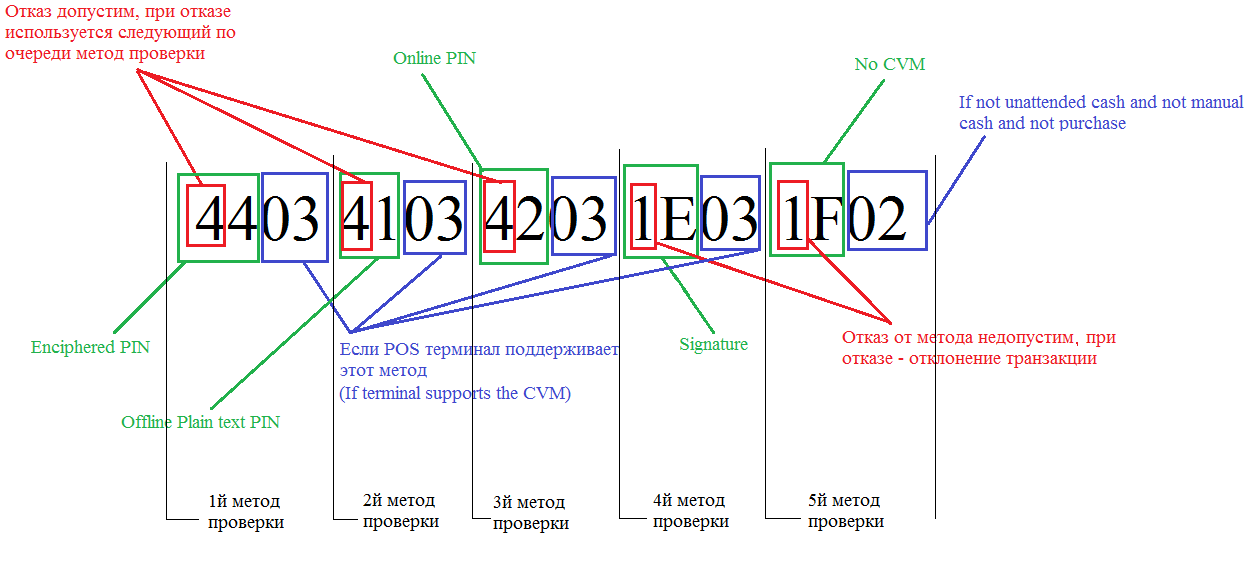
\includegraphics[width=0.9\textwidth]{images/research/cvm_check}
    \caption{\centering Расшифрока CVM списка}
    \label{fig:cvm_check}
\end{figure}

Данному примеру соответствует следующий алгоритм действий (при условии совпадения наличия методов):

\begin{enumerate}
    \item запрос PIN карты,
    \item если пользователь отказывается (а он имеет право отказаться)~--- запрос открытого офлайн-PIN,
    \item если снова отказывается~--- запрос онлайн-PIN, который проверяется не картой, а хостом,
    \item если снова отказался~--- запрос подписи (от ее ввода уже невозможно отказаться).
\end{enumerate}

Если в CVM-листе терминала не указан метод <<проверка по подписи>>~--- тогда он пропускается, и это не приравнивается к отказу выполнения транзакции, потому что в таком случае используется метод <<No CVM>> с условием «If not unattended cash and not manual cash and not purchase».
Если и этого метода в CVM-листе терминала нет~--– то проверка неудачная и транзакция отклоняется~\cite{habr_cvm}.


\subsection{Стандарт бесконтактного интерфейса ISO/IEC 14443}
\label{subsec:iso_14443}

ISO/IEC 14443 - это международный стандарт, описывающий требования к технологиям бесконтактной идентификации, используемой в смарт-картах и
RFID-устройствах. 
Этот стандарт охватывает физические характеристики карт, протоколы передачи данных и методы антиколлизии~\cite{iso_14443}.
Основное применение данный стандарт нашел в сфере бесконтактных платежей посредством банковских карт.
Помимо этого он используется в электронных проездных, а также удостоверениях личности и электронных паспортах.

Обмен информации основан на принципе индуктивной связи между антенной модуля и антенной карты.
Под антенной понимается замкнутая металлическая катушка, способная принимать и излучать электромагнитные волны.
Дальность взаимодействия бесконтактной связи составляет до 10 см, а скорость передачи данных варьируются в диапазон от 106 до 848 кбит/с.
Данный стандарт входит в состав технологии NFC, структура которого представлена на рисунке~\ref{fig:nfc_tech}, там же изображено разделение технологии на различные слои, начиная с физического уровня и заканчивая уровнем приложений (снизу вверх).

\begin{figure}[H]
    \centering
    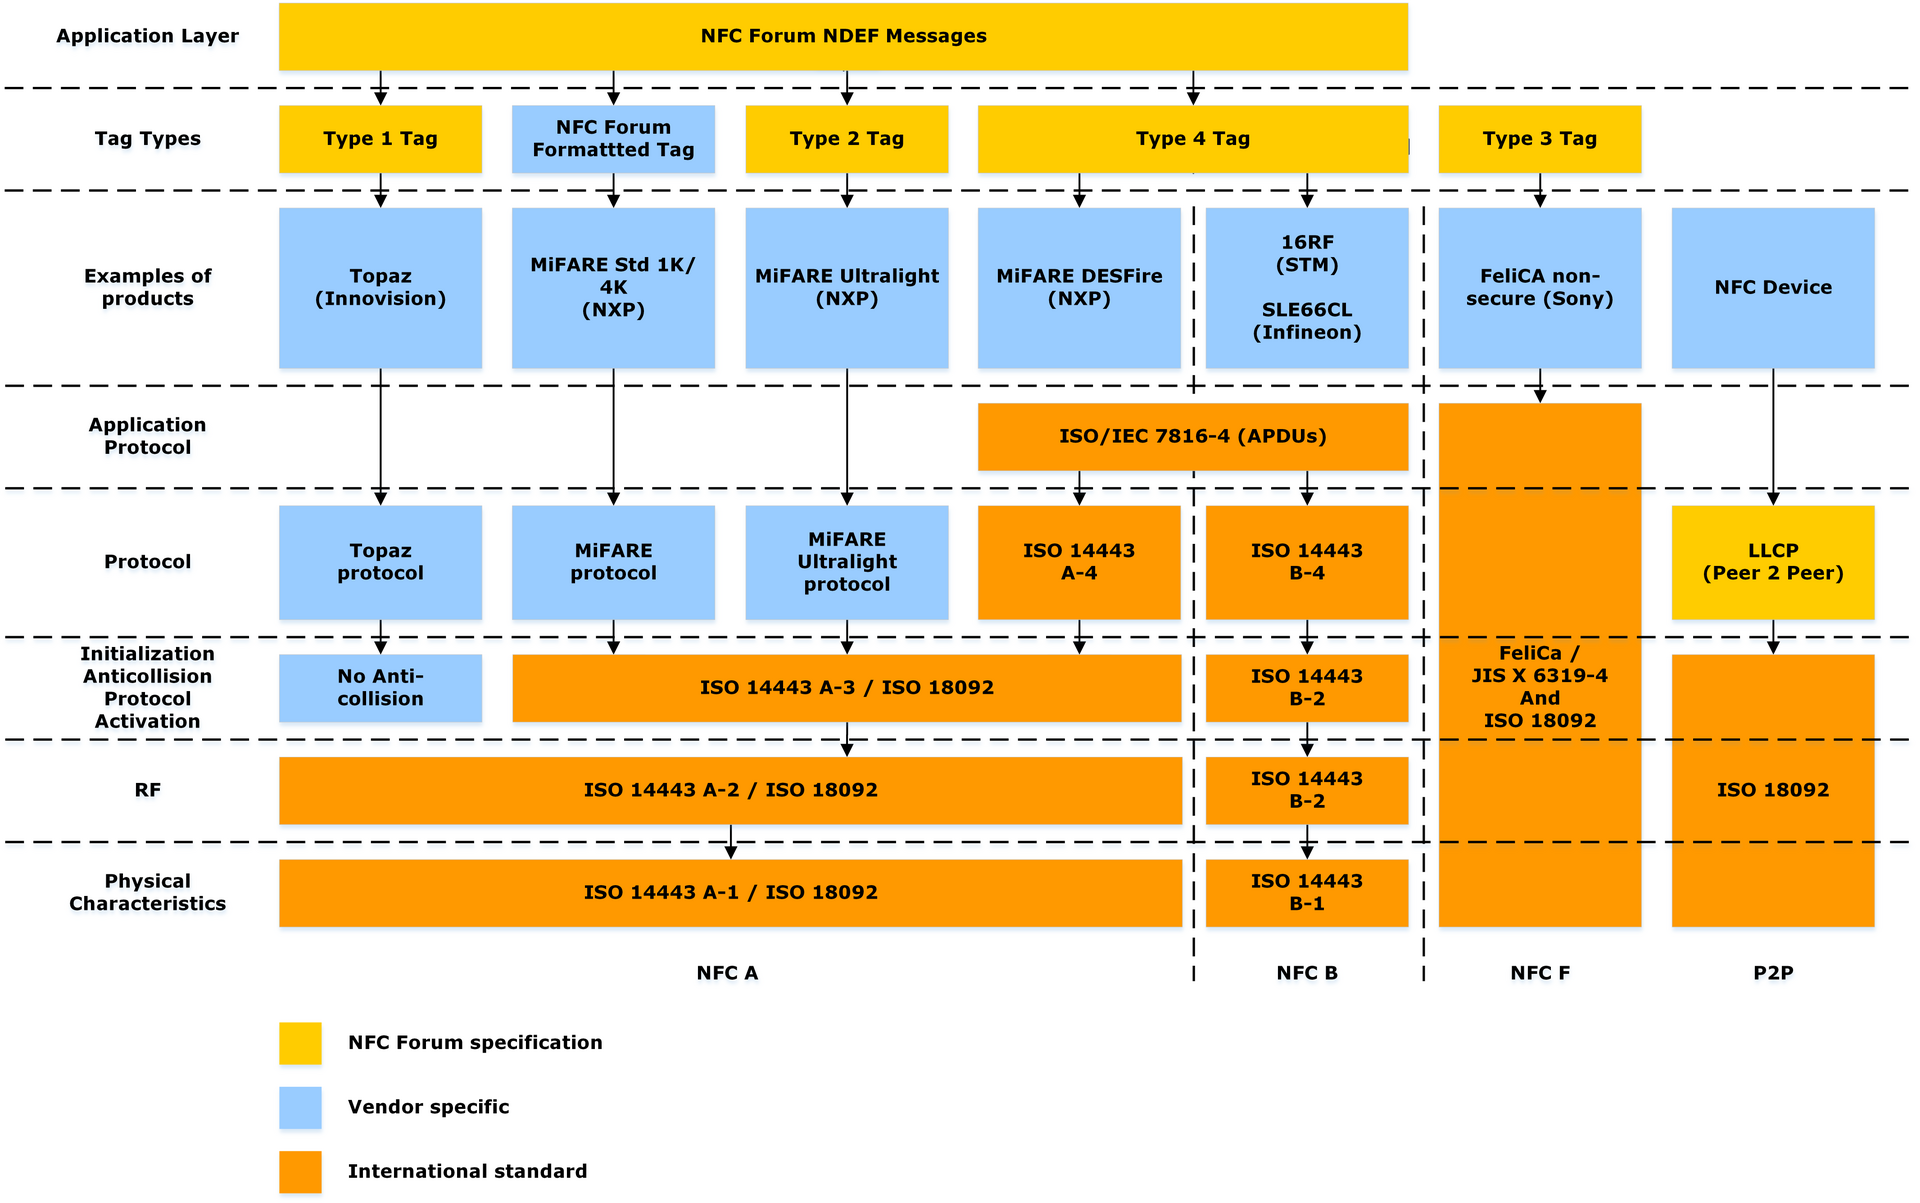
\includegraphics[width=1\textwidth]{images/research/nfc_tech}
    \caption{\centering Стек протоколов NFC}
    \label{fig:nfc_tech}
\end{figure}

Каждый из описанных уровней связан с определёнными стандартами и обеспечивает целостность работы технологии NFC, начиная с физической передачи сигнала и заканчивая выполнением прикладных задач.

Near-field communication (NFC) - это технология беспроводной связи малого радиуса действия, которая позволяет передавать данные между двумя устройствами, находящимися на расстоянии до 20 сантиметров.
Данная технология представляет собой набор протоколов связи, которые обеспечивают низкоскоростное соединение с простым и быстрым подключением.
Подобно другим технологиям карт ближнего взаимодействия, NFC основана на индуктивной связи между двумя электромагнитными катушками, встроенными в устройства с поддержкой NFC, такие как смартфоны.
Для обмена данными в одном или обоих направлениях NFC использует частоту 13,56 МГц, находящуюся в глобально доступном нелицензируемом диапазоне ISM (Industrial, Scientific and Medical).
NFC имеет собственную стандартизацию ISO/IEC 18000--3~\cite{nfc_wiki}.

Она охватывает как протоколы связи, так и форматы обмена данными, которые основаны на существующих стандартах радиочастотной идентификации (RFID), в частности ISO/IEC 14443, благодаря поддержке которого получила широкое применение в сфере бесконтактной оплаты.
Важно, что данная технология реализует также ISO/IEC 7816~--- это позволяет устройствам, содержащим модуль NFC 4-го типа (NFC Type 4 Tag) использоваться для бесконтактной оплаты, т.к. данные модули совместимы с терминалами оплаты.

ISO 14443 разделяется на четыре части:

\begin{enumerate}
    \item физические характеристики: содержит описание размеров, материалов и формы карт (обычно формата ID-1, аналогичного банковским картам);
    \item радиоинтерфейс: определяет электромагнитные параметры, включая метод модуляции и демодуляции сигнала;
    \item инициализация и методы антиколлизии: описывает, как карты идентифицируются, и как модуль выбирает конкретную карту из множества доступных (например, в очереди пользователей);
    \item протокол обмена данными: устанавливает правила взаимодействия между картой и модулем, включая форматы команд и структуру данных, содержит описание Half-duplex block transmission protocol~--- протокола, разработанного в соответствии с принципом многоуровневости модели OSI, предназначенного для минимизации взаимодействия карты и модуля, описывая правила между границами уровней данной модели и количества уровней~\cite{iso_14443_en}.
\end{enumerate}


На данный момент существует 2 версии данного стандарта: A и B.
Изначально был разработан стандарт А, однако он обладал недостатками в виде ограниченной производительности и совместимости.
Версия B была разработана позже с целью их исправления.
Устройство на базе версии B данного стандарта обладает большей технической сложностью, а его стоимость выше, чем у устройств ана базе версии A.
Поэтому наиболее широкое применение по-прежнему остается за стандартом A.
Именно он используется в сфере банковских платежей с помощью бесконтактных карт.
Тип B чаще используется в более сложных системах, где необходимо передавать больший объем данных, и имеется больше требований безопасности.
Примерами таких систем выступают:

\begin{itemize}
    \item электронные паспорта (ePassports),
    \item удостоверения личности,
    \item медицинские карты.
\end{itemize}

Основные отличия технологий A и B приведены в таблице~\ref{tab:iso14443_comparison}.

\begin{longtable}[l]{|
P{0.3\textwidth}|
P{0.33\textwidth}|
P{0.3\textwidth}|}

    \caption{Сравнительная характеристика стандартов ISO 14443-A и ISO 14443-B}
    \label{tab:iso14443_comparison} \\
    \hline
    \textbf{Характеристика} &
    \textbf{ISO 14443-A} &
    \textbf{ISO 14443-B} \\
    \hline
    \endfirsthead

    \caption*{Продолжение таблицы~\ref{tab:iso14443_comparison}} \\
    \hline
    \textbf{Характеристика} &
    \textbf{ISO 14443-A} &
    \textbf{ISO 14443-B} \\
    \endhead

    \endfoot

    \endlastfoot

    Метод модуляции &
    Amplitude Shift Keying (ASK) &
    Binary Phase Shift Keying (BPSK) \\
    \hline

    Скорость передачи &
    106 кбит/с &
    106, 212, 424, 848 кбит/с \\
    \hline

    Антиколлизия &
    метод <<первый пришёл~-- первый вышел>> &
    временные слоты и уникальные идентификаторы \\
    \hline

    Стабильность питания &
    низкая &
    высокая \\
    \hline

    Устойчивость к помехам &
    высокая защита от помех &
    уязвимость к внешним воздействиям \\
    \hline
\end{longtable}


ISO/IEC 14443--3 (третий уровень стандарта ISO/IEC 14443) фокусируется на установлении связи между устройствами считывания (PCD - Proximity Coupling Device) и бесконтактными картами (PICC - Proximity Integrated Circuit Card).
Данный уровень определяет механизмы обнаружения карт, установления связи и антиколлизии.
Этот уровень является критически важным для правильной работы систем, где одновременно могут находиться несколько карт в зоне действия ридера~\cite{iso14443-3}.

Антиколлизия (anti-collision) в контексте стандарта ISO/IEC 14443-3~--- это механизм, позволяющий устройству чтения (PCD) корректно идентифицировать и взаимодействовать только c одной картой (PICC) в случае, когда несколько бесконтактных карт находятся в зоне действия считывателя.

Стандарт ISO/IEC 14443--3 описывает следующие аспекты взаимодействия PCD и PICC:

\begin{itemize}
    \item процесс обнаружения карт (Polling): обнаружение карт PCD, которые входят в поле его действия;
    \item формат байтов, кадры и временные характеристики: правила формирования кадров данных и временные интервалы передачи, которые должны соблюдаться для корректной передачи информации между устройствами;
    \item антиколлизионные методы: способы обнаружения и выбора одной карты из нескольких, находящихся в зоне действия ридера;
    \item инициализация связи: начальная команда запроса, корректный ответ на запрос и ошибки соединения, а также параметры, необходимые для начала взаимодействия между PCD и PICC.
\end{itemize}

В соответствии со стандартом определена диаграмма состояний бесконтактной карты, представленная на рисунке~\ref{fig:picc_states}, она является конечным автоматом.

\begin{figure}[H]
    \centering
    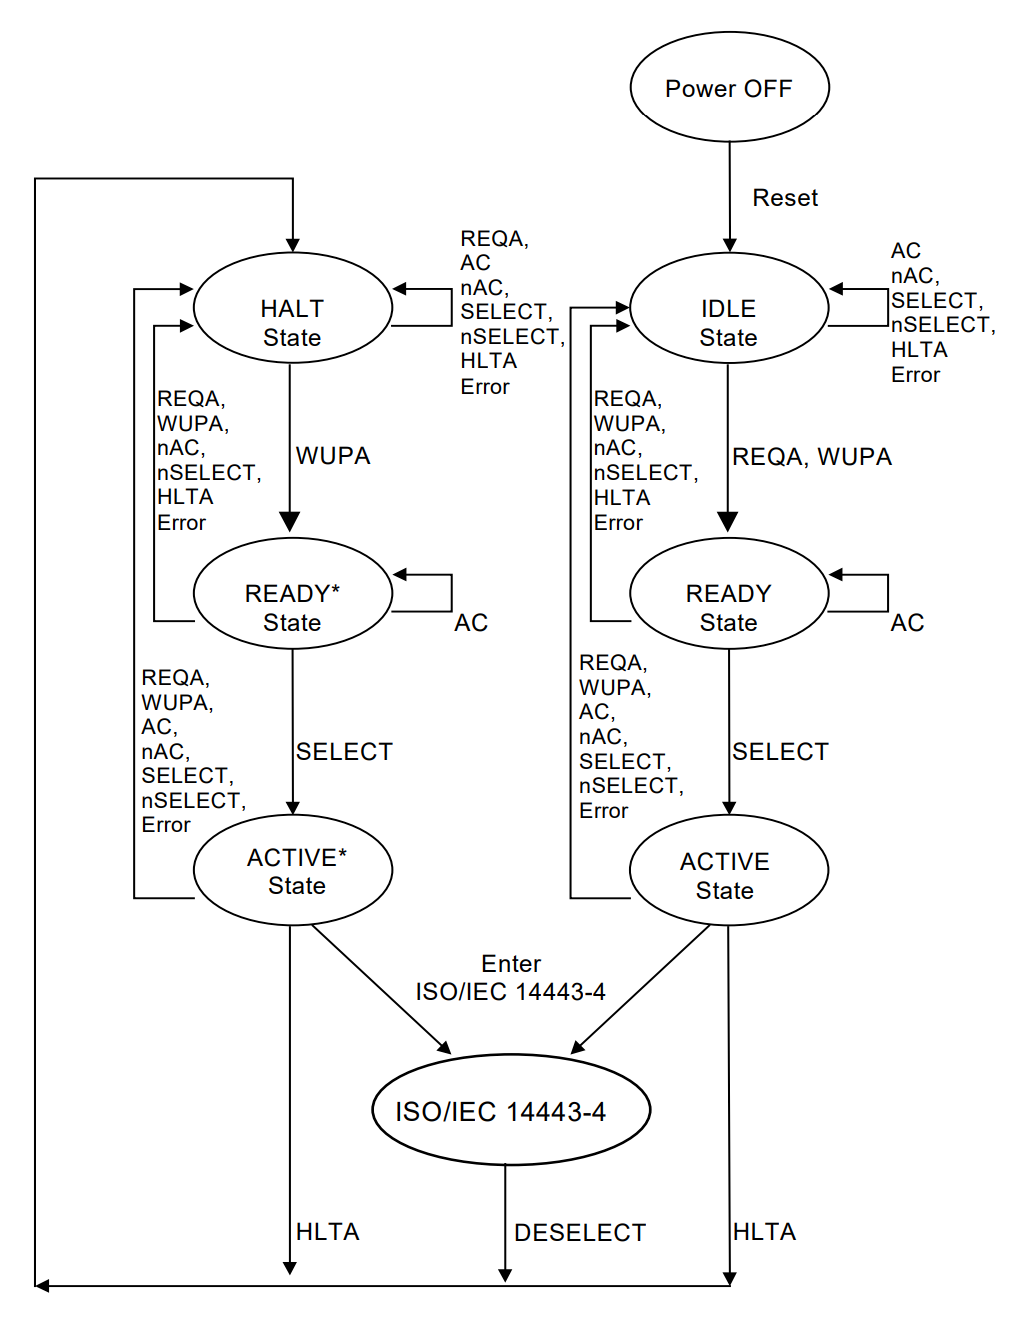
\includegraphics[width=0.5\textwidth]{images/research/picc_states}
    \caption{\centering Диаграмма состояний бесконтактой карты с интегральной схемой}
    \label{fig:picc_states}
\end{figure}

Как видно из рисунка~\ref{fig:picc_states}, бесконтактная карта с интегральной схемой имеет несколько основных состояний:

\begin{itemize}
    \item Power OFF: состояние выключения,
    \item IDLE и HALT: состояния ожидания, которым свойственно низкое потребление электроэнергии,
    \item READY и READY*: состояния готовности к работе,
    \item ACTIVE и ACTIVE*: основные рабочие состояния, в которых доступен функционал, описанный в ISO 14443--4.
\end{itemize}

Также в соответствии со стандартом определен алгоритм работы устройства PCD, который представлен на рисунке~\ref{fig:pcd_flow}.
На нем изображена последовательность работы устройства считывания.

\begin{figure}[H]
    \centering
    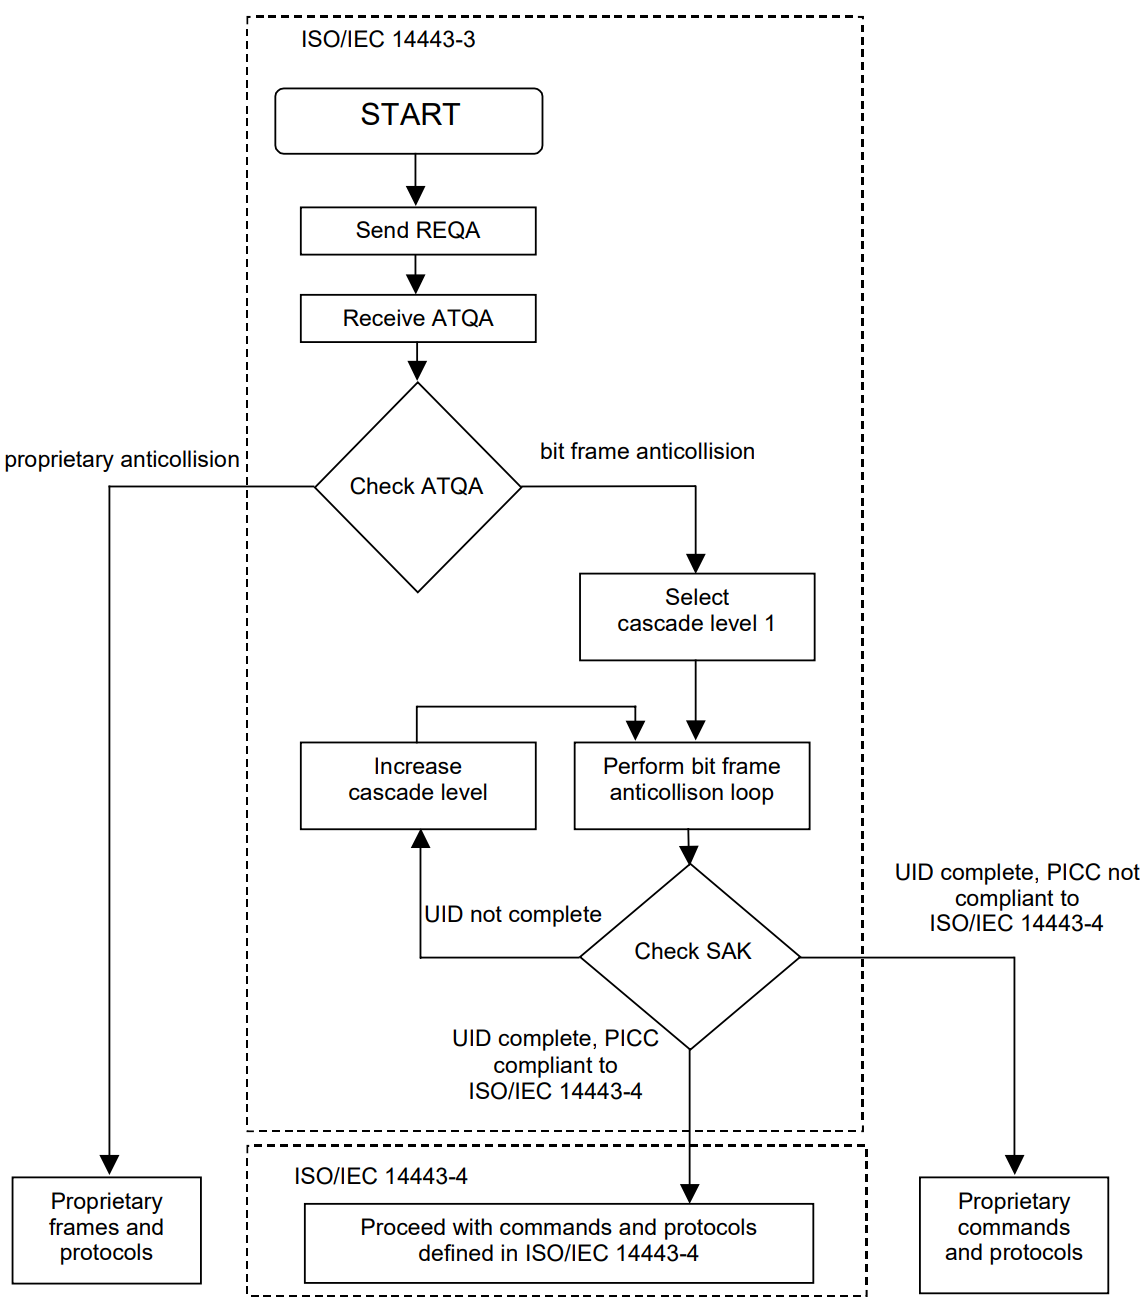
\includegraphics[width=0.7\textwidth]{images/research/pcd_flow}
    \caption{\centering Алгоритм работы устройства-считывателя}
    \label{fig:pcd_flow}
\end{figure}


На рисунках~\ref{fig:picc_states} и~\ref{fig:pcd_flow} приводятся следующие команды и процедуры, с помощью которых происходит взаимодействия PICC и PCD (приписка <<A>> обозначает, что данная команда предназначена для карт, взаимодействующих по стандарту ISO/IEC 14443-A):

\begin{itemize}
    \item REQA (Request A)~--- команда, отправляемая устройством считывания (PCD) для инициирования взаимодействия с картой (PICC), находящейся в состоянии <<IDLE>>, предназначена для проверки наличия карты в пределах досягаемости;
    \item WUPA (Wake-Up A)~--- команда для пробуждения карты из состояния <<HALT>>, используется, если карта находится в режиме ожидания и должна быть возвращена в активное состояние;
    \item AC (Anti-collision)~--- процедура антиколлизии, используемая для выбора одной карты из нескольких, находящихся в зоне действия устройства считывания, позволяет идентифицировать уникальный идентификатор карты (UID);
    \item nAC (Negative Anti-collision)~--- действие обратное процедуре антиколлизии, указывающее, что карта не была выбрана или произошла ошибка во время антиколлизионного процесса;
    \item SELECT~--- команда выбора карты, завершает процесс антиколлизии и устанавливает карту в активное состояние, после выполнения этой команды карта готова к обмену данными;
    \item nSELECT (Negative Select)~--- отрицательная команда выбора, применяемая при ошибке во время процесса выбора карты;
    \item HLTA (Halt A)~--- команда, переводящая карту в состояние <<HALT>>, в этом состоянии карта не отвечает на команды до получения команды WUPA;
    \item Error~--- состояние или ответ, возникающий в случае некорректного выполнения команды или нарушения последовательности команд;
    \item DESELECT~--- команда для завершения активного состояния карты, переводя её обратно в состояние <<IDLE>>;
    \item Enter ISO/IEC 14443--4~--- процесс, переводящий карту в следующий уровень протокола -- ISO/IEC 14443--4.
\end{itemize}


ISO/IEC 14443--4 описывает полудуплексный протокол передачи данных блочного типа (half-duplex block transmission protocol).
В данном стандарте определяются последовательности активации и деактивации протокола, а также обеспечивается взаимодействие с другими частями стандарта ISO/IEC 14443.

В данной части стандарта описана поддержка передачи блоков данных прикладного уровня (Application Protocol Data Units, APDUs), описанных в ISO/IEC 7816--4.
Что позволяет осуществлять сопоставление данных в формате APDU и использовать механизмы выбора приложений в соответствии с ISO/IEC 7816--5~\cite{iso_14443_en}.

В данной части протокола подробно описана активация PICC с помощью устройства PCD, схема активации приведена на рисунке~\ref{fig:pcd_flow_2_picc_activation}.


\begin{figure}[H]
    \centering
    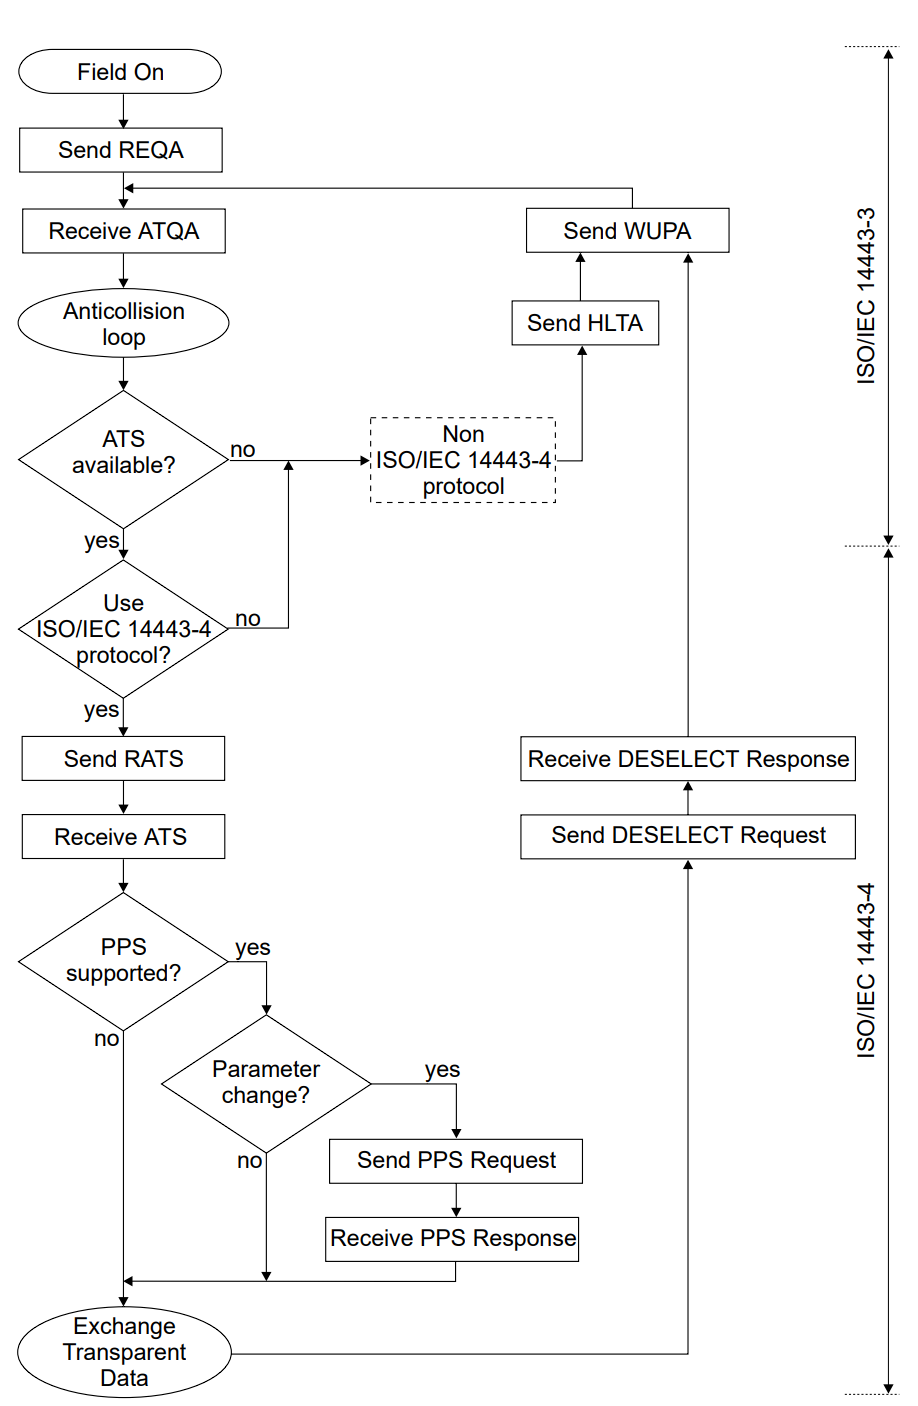
\includegraphics[width=0.7\textwidth]{images/research/pcd_flow_2_picc_activation}
    \caption{\centering Активация бесконтактной карты с помощью PCD}
    \label{fig:pcd_flow_2_picc_activation}
\end{figure}

Данный алгоритм в дополнение к действия, рассмотренным в ISO/IEC 14443--3, описывает действия, которые необходимо сделать для активации полудуплексного протокола передачи данных.
Важно отметить, что отправка RATS (Request for Answer To Select) на PCD в качестве следующей команды происходит после получения SAK, а также, что PICC отвечает на RATS~--- ATS (Answer To Select), это происходит только в том случае, если RATS получен непосредственно после выбора PICC.

Каждый бит RATS, ATS, PPS детально описан в 5 разделе ISO 14443--4~\cite{iso14443-4} Однако дополнительная информация также содержится в спецификации бесконтактного взаимодействия по стандарту EMV, в частности в разделе 10~\cite{emv_specifications_book}.

Half-duplex block transmission protocol~--- полудуплексный протокол передачи данных в виде блоков (кадров).
Он учитывает особые потребности внешнего окружения бесконтактных карт и использует определенный формат кадра, представленный на рисунке~\ref{fig:hd_block_format}.
Кадр состоит из поля пролога (обязательного), информационного поля (необязательного) и поля эпилога (обязательного).

\begin{figure}[H]
    \centering
    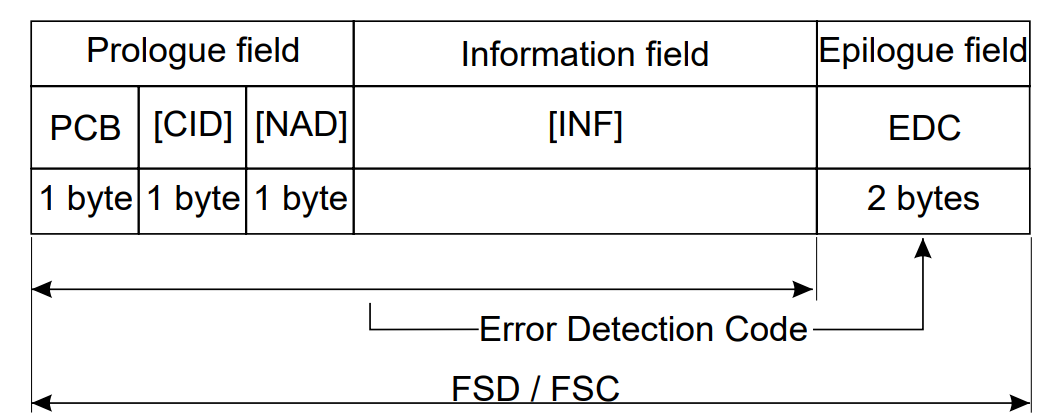
\includegraphics[width=0.5\textwidth]{images/research/hd_block_format}
    \caption{\centering Стандартный формат кадра Half-duplex block transmission protocol}
    \label{fig:hd_block_format}
\end{figure}

Каждый бит элементов данного кадра детально описан в 7 разделе ISO 14443--4~\cite{iso14443-4}.
Дополнительная информация, также содержится в спецификации стандарта EMV, в частности в разделе 10~\cite{emv_specifications_book}.


\subsection{Стандарт контактного интерфейса ISO/IEC 7816}
\label{subsec:7816}

ISO/IEC 7816~--- это международный стандарт, который регулирует использование интегрированных схем (ИС) в картах, известных как смарт-карты.
Он охватывает различные аспекты смарт-карт, включая их физические характеристики, электрические интерфейсы, протоколы передачи данных и др..
Стандарт состоит из 15 частей, каждая из которых фокусируется на каком-либо аспекте~\cite{7816_wiki}.

Основное преимущество стандарта ISO/IEC 7816~--- способность обеспечивать совместимость между продуктами различных производителей.
Это достигается благодаря четким спецификациям, которые позволяют разработчикам создавать устройства и приложения, совместимые с картами, соответствующими этому стандарту.
В рамках данного стандарта описывается формат взаимодействия с картой на уровне приложения с помощью APDU.

\subsubsection{Формат APDU}

APDU (Application Protocol Data Unit)~--- это формат команд и ответов, используемый для взаимодействия между считывателями карт, например, платежными терминалами, и смарт-картами, в том числе банковскими картами с поддержкой технологии EMV.
Команды данного формата определены в стандарте ISO/IEC 7816 и разделены на два типа:

\begin{itemize}
    \item Command APDU~--- команда от терминала к карте;
    \item Response APDU~--- ответ от карты терминалу.
\end{itemize}


APDU-команды используются для передачи инструкций, таких как выбор приложения, запрос информации о карте, выполнение транзакций, чтение данных, а также запись информации на карту.
Важно отметить, что за счет APDU протокол ISO/IEC 7816 позволяет взаимодействовать с контактными картами как и с бесконтактными, посредством использования определенных команд.
Такая гибкость использования стандарта достигается за счет абстрагирования над другими протоколами взаимодействия, упомянутых в предыдущих разделах.

Команда APDU состоит из двух основных компонентов: заголовок и данные.
Более детальная структура представлена на рисунке~\ref{fig:apdu_com}.

\begin{figure}[H]
    \centering
    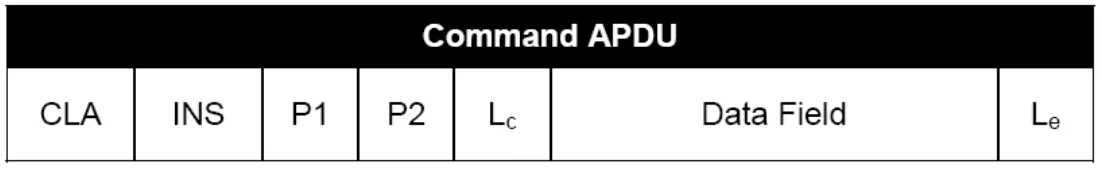
\includegraphics[width=0.7\textwidth]{images/research/apdu_com}
    \caption{\centering Структура APDU команды}
    \label{fig:apdu_com}
\end{figure}


APDU команда (APDU Command) разделяется на следующие элементы~\cite{medium_apdu2}:

\begin{itemize}
    \item CLA (Class): класс инструкции, определяет класс команды и используется для указания типа команды, которую карта должна выполнить;
    \item INS (Instruction): тип инструкции (например, SELECT, READ RECORD), определяет конкретную команду, которую должна выполнить карта;
    \item P1 и P2: параметры для команды (например, указание файла, записи), предоставляют дополнительную информацию или данные для адресации внутри карты;
    \item Lc: длина поля данных команды, если данные присутствуют (необязательный элемент);
    \item  Data (если применимо для команды): данные, специфичные для команды, которые необходимо отправить на карту (например, идентификатор приложения);
    \item Le: ожидаемая длина ответа от карты (необязательный элемент).
\end{itemize}


Структура APDU ответа (APDU Response) представлена на рисунке~\ref{fig:apdu_resp}.

\begin{figure}[H]
    \centering
    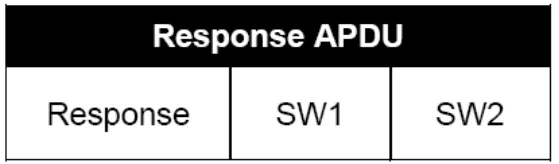
\includegraphics[width=0.5\textwidth]{images/research/apdu_resp}
    \caption{\centering Структура APDU ответа}
    \label{fig:apdu_resp}
\end{figure}

В состав APDU ответа входят следующие элементы:

\begin{itemize}
    \item Data: данные, отправленные картой в ответ на команду;
    \item SW1 и SW2 (Status Words): двухбайтовые коды статуса, указывающий результат выполнения команды.
\end{itemize}

Наиболее распространенными ответами являются <<90:00>>, означающий успешное выполнение, и <<6A:82>>~-- ошибка поиска файла или приложения~\cite{iso7816-4}.


\subsubsection{Прикладное применение APDU}

Для инициализации транзакции между картой и терминалом, обмена данными и завершения процесса необходимо следовать определенной последовательности APDU команд.

Cписок стандартных APDU команд ISO 7816--4, в т.ч. используемых в стандарте EMV, приведен на рисунке~\ref{fig:apdu_commands}~\cite{iso7816-4}.

\begin{figure}[H]
    \centering
    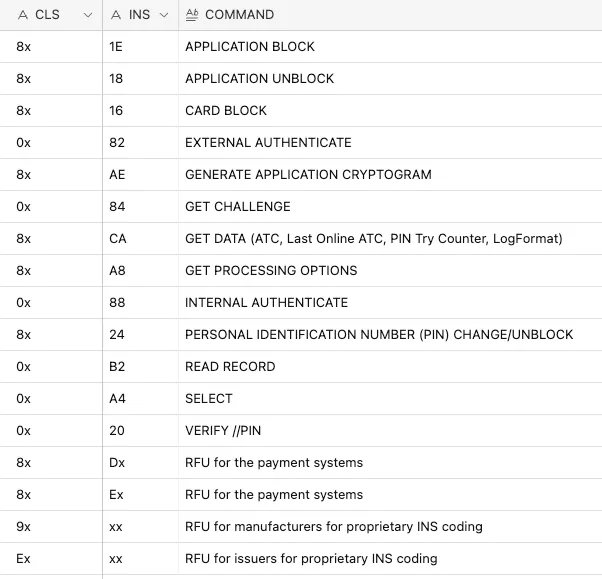
\includegraphics[width=0.7\textwidth]{images/research/apdu_commands}
    \caption{\centering Список APDU команд, используемых при взаимодействии карты и терминала}
    \label{fig:apdu_commands}
\end{figure}

APDU-команды могут быть использованы для выбора приложения на банковской карте и для последующей работы с ним.
Есть приложения, в т.ч. платежные, которые способны взаимодействовать с данными в памяти карты.
С их помощью можно запросить информацию, содержащую различные данные карты, например ее срок действия карты, уникальный номер и пр.
Таким образом во время выполнения платежной транзакции получаются все необходимые данные.
Для подобных целей обычно используется команда READ RECORD, после предварительного выбора приложение для работы с памятью по его AID.
Для выбора конкретного приложения необходимо указать AID (Application Identifier) при использовании команды SELECT.
В ответе на данную команду карта сообщает об успешном или неуспешном выборе приложения~\cite{medium_apdu2_1}.



\subsection{Стандарт EMV Contactless}

% EMV Transaction Flow - стр. 29
% активация ISO 14443-4 - стр. 43

Для осуществления бесконтактной оплаты платежная карта должна соответствовать <<EMV Level 1 Specifications for Payment Systems, EMV Contactless Interface Specification>>.
Транзакция может быть инициирована ТСП, как правило, путем ввода суммы транзакции или после того, как карта была внесена в радиочастотное поле терминала и указала на свое присутствие, отправив сигнал терминал.
Транзакция продолжается до тех пор, пока держателю карты не будет указано окончательное результат ее выполнения.
Это может быть сразу после обработки платежным ядром для офлайн-одобрения или отклонения или после получения ответа авторизации, если транзакция отправляется онлайн.
Если требуется дальнейшее взаимодействие терминала с картой, то это тоже часть транзакции~\cite{emv_book_A}.


\subsubsection{Архитектура бесконтактного POS-терминала}

Есть 3 различные архитектуры POS-терминала:
\begin{itemize}
    \item изолированный POS-терминал~--- все элементы в одном устройстве;
    \item продвинутый считыватель карт~--- внешнее устройство <<терминал>> в малой степени участвует в выполнении транзакции, получая данные от считывателя, который выполняет большую часть взаимодействия для выполнения транзакции;
    \item комбинация устройства-терминала и <<прозрачного>> считывателя карт~--- транзакция выполняется на устройстве <<терминале>>, считыватель используется только для взаимодействия с картой.
\end{itemize}

По данной классификации разрабатываемое устройство является продвинутым считывателем карт.

Основные функции POS-системы включают:
\begin{itemize}
    \item связь с бесконтактными картами,
    \item выбор платежного приложения на карте и активация платежного ядра на терминале,
    \item отображение сообщений держателю карты,
    \item отображение сообщений продавцу,
    \item прием ввода данных ТСП о сумме транзакции,
    \item проверка держателя карты (например, ввод PIN-кода),
    \item предоставление онлайн-подключений,
    \item предоставление сбора данных для клиринга и расчетов
\end{itemize}

Важную роль в выполнении транзакции играет Entry Point~--- специальное ПО в системе оплаты, которое выполняет следующие функции:
\begin{itemize}
    \item препроцессинг или предварительная обработка перед установкой взаимодействия карты и терминала;
    \item обнаружение карты, установка связи с ней по стандарту ISO/IEC 14443;
    \item выбор бесконтактного приложения, поддерживаемого как картой, так и считывателем;
    \item активация соответствующего платежного ядра (разные ПС имеют разные платежные ядра);
    \item обработку результатов, возвращаемых ядром, включая передачу выбранных результатов считывателю.
\end{itemize}

Платежное ядро (Kernel)~--- специальное ПО для выполнения бесконтактных платежных транзакций.
Детально описаны в <<EMV Contactless Specifications for Payment Systems>> книгах С-n.
Формирует некий результат (Outcome), который позволяет Entry Point определить статус выполнения транзакции для дельнейшего взаимодействия с пользователем.

Модели POS-терминала для бесконтактной оплаты представлен на рисунке~\ref{fig:pos_design_example}.
Данная модель в стандарте приводится для примера, т.к. возможно иное распределение функционала между терминалом и считывателем~\cite{emv_book_A}.

\begin{figure}[H]
    \centering
    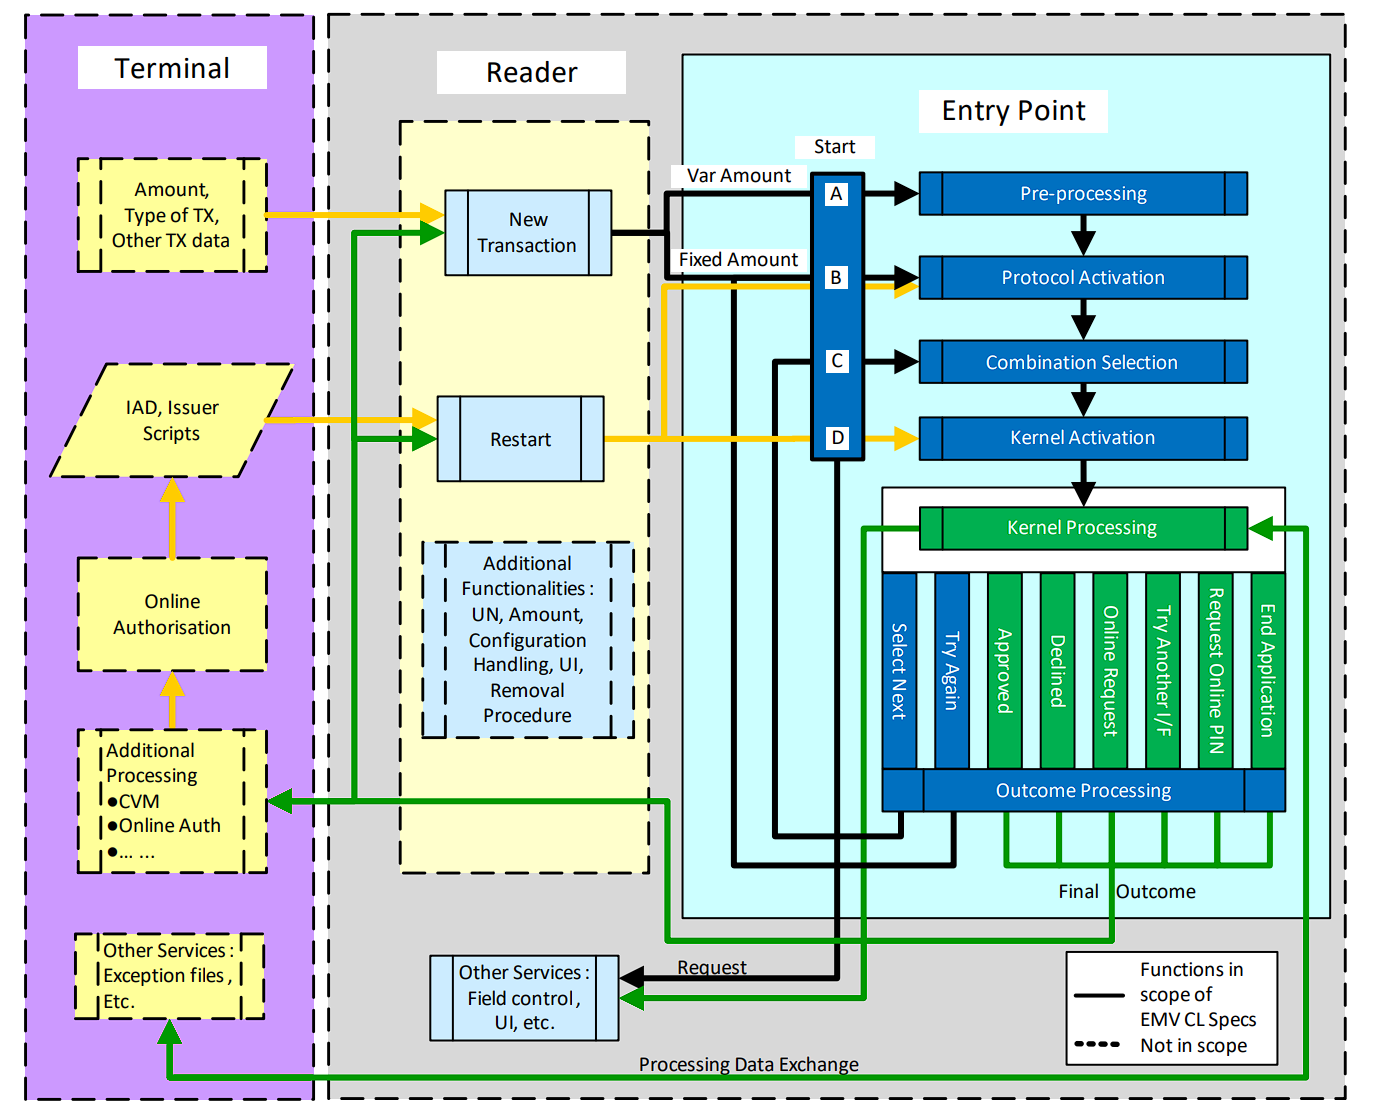
\includegraphics[width=0.7\textwidth]{images/research/pos_design_example}
    \caption{\centering Архитектура POS-терминала бесконтактной оплаты}
    \label{fig:pos_design_example}
\end{figure}

%Онлайн-авторизация либо приведет к ответу с кодом ответа и возможными данными EMV TLV, либо истечет время ожидания и будет считаться неспособным выйти в сеть.
%В средах режима EMV типичными элементами данных EMV TLV, которые могут присутствовать, являются код ответа авторизации (тег '8A'), данные аутентификации эмитента (тег '91') и шаблон сценария эмитента (тег '71', '72')


\subsubsection{Выполнении бесконтактной транзакции}

% дальше написано по book_A
При выполнении бесконтактной транзакции POS-системе может потребоваться проверка держателя карты, чтобы убедиться, что лицо, предъявляющее карту, является ее держателем, подробно данные проверки рассматривалась в пункте~\ref{subsubsec:transaction_security_check}.
Для бесконтактной транзакции могут выполняться следующие проверки:

\begin{itemize}
    \item проверка PIN-кода держателя карты посредством онлайн проверки банком (Online PIN);
    \item получение кода подтверждения транзакции посредством пройденной проверки на устройстве держателя карты (например, посредством ввода отпечатка пальца на смартфоне, используемом для оплаты);
    \item запрос подписи держателя карты (либо печать чека со строкой для подписи, либо ввод подписи посредством сенсорного экрана)~\cite{emv_book_A}.
\end{itemize}

Проверка PIN-кода не выполняется офлайн из-за временных ограничений по операциям с картой в поле.
При конфигурации POS-терминала указывается следующее:

\begin{itemize}
    \item страна и поддерживаемые валюты платежей (Terminal Country Code~-- тег <<9F1A>>, Transaction Currency Codes~-- тег <<5F2A>>);
    \item индикатор начала транзакции (действием держателя терминала, например вводом суммы, или автоматически при обнаружении карты);
    \item поддерживаемые способы оплаты картой (магнитной полосой, контактным или бесконтактным чипом);
    \item поддерживаемые типы транзакций (онлайн и/или офлайн);
    \item данные конфигурации ядра и Entry Point для различных комбинаций типа транзакции, платежного приложения и ядра~\cite{emv_book_A}.
\end{itemize}

% дальше написано по kernel_8
Процесс выполнение транзакции отличается в зависимости от используемого платежного ядра.
Разные ПС используют разные ядра для обработки транзакций с картами, поскольку процесс обработки транзакции по ним может отличаться.
Стандарт EMV предлагает общий алгоритм выполнения платежной транзакции в спецификации на Kernel 8, он представлен на рисунке~\ref{fig:kernel_transaction_flow}~\cite{emv_book_c8}.

\begin{figure}[H]
    \centering
    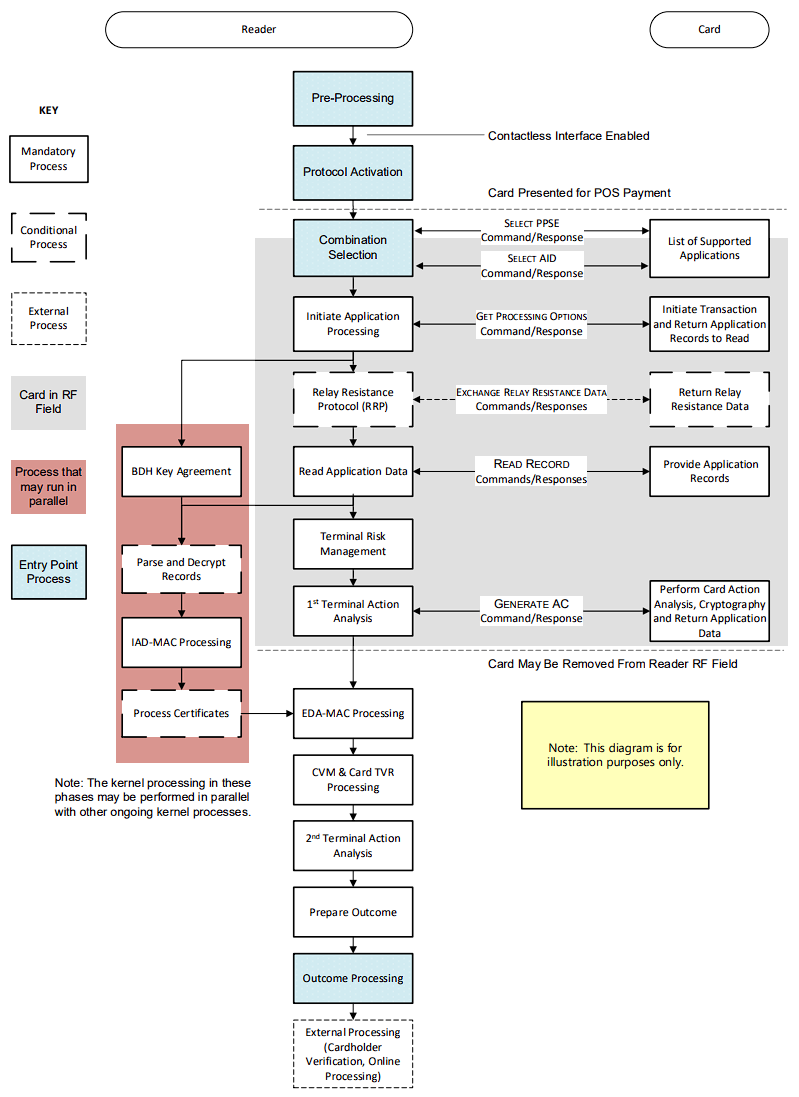
\includegraphics[width=0.8\textwidth]{images/research/kernel_transaction_flow}
    \caption{\centering Пример выполения бесконтактной траназкции}
    \label{fig:kernel_transaction_flow}
\end{figure}

Данный алгоритм отличается для разных платежных ядер, но позволяет сформировать понимание процессов, происходящих во время выполнения бесконтактной оплаты.

Предварительная обработка (Pre-Processing) обычно выполняется для новых транзакций с переменной суммой.
В некоторых реализациях, например, когда считыватель обрабатывает фиксированную сумму транзакции, предварительная обработка может не потребоваться, и транзакция может начаться при активации протокола.
Выполнение данного этапа рассмотрено в пункте~\ref{subsubsec:pre-processing}.

Во время активация протокола (Protocol Activation) считыватель опрашивает на наличие бесконтактных карт, которые могли попасть в радиочастотное поле считывателя, данный процесс описан в подразделе~\ref{subsec:iso_14443}.
Он заканчивается выбором карты для взаимодействия и выполнения платежа.
Выполнение данного этапа рассмотрено в пункте~\ref{subsubsec:protocol_activation}.

В процессе выбора комбинации (Combination Selection) происходит взаимодействие с картой в ходе которого выполняется выбор комбинации платежного ядра и приложения, которые будут поддерживаться картой и терминалом.

Во время первичной обработки приложения (Initiate Application Processing) платежное ядро подает сигнал карте о начале обработки транзакции, отправляя команду GET PROCESSING OPTIONS (GPO) карте.
При выдаче этой команды ядро предоставляет карте любые объекты данных, запрошенные картой в списке объектов данных параметров обработки (Processing Options Data Object List~-- PDOL).

Согласование ключей с помощью криптографического протокола Диффи-Хеллмана с обфусцированным публичным ключом (BDH Key Agreement), использование протокола сопротивления ретрансляции (Relay Resistance Protoco~-- RRP) используется для повышения безопасности транзакции конкретно в рамках Kernel~8.

На этапе Read Application Data платежное ядро запрашивает у карты данные, необходимые для завершения транзакции.
После получения ответа на команду GET PROCESSING OPTIONS (GPO), или RRP, если она поддерживается, Kernel проверяет, какие именно данные нужно прочитать согласно указаниям в Application File Locator (AFL).
Ядро последовательно отправляет команды READ RECORD для получения всех указанных записей, среди которых может быть информация о владельце, параметрах аутентификации и других реквизитах~\cite{emv_book_c8}.

После того, как ядро получит необходимые данные из предыдущих шагов для продолжения, оно выполняет анализ рисков транзакции (Terminal Risk Management) для определения параметров CVM считывателя, выполняет проверки floor limit and CVM limit и может инициировать локальную аутентификацию, если она поддерживается и включена.

На этапе Card Action Analysis, карта получает команду GENERATE AC от платежного ядра (Kernel) и выполняет собственный анализ транзакции.
Этот шаг является ключевым для завершения аутентификации карты и принятия решения о результате операции.
Карта проводит проверки:

\begin{itemize}
    \item проверяет что не нарушены ограничения по сумме, условия использования карты и другие бизнес-правила;
    \item выполняет карточную верификацию (CVM decisioning): определяет требуется ли ввод PIN-кода или можно продолжить транзакцию без дополнительной проверки и формирует решение по транзакции: одобрить офлайн, запросить онлайн-авторизацию, отклонить или переключиться на другой интерфейс (например, контактный);
    \item генерирует IAD-MAC (код целостности данных транзакции), EDA-MAC (улучшенная подпись для аутентификации) и Application Cryptogram~--- криптограмму, подтверждающую легитимность транзакции.
\end{itemize}

Ответ карты содержит информацию, необходимую платежному ядру для дальнейшей обработки транзакции, включая тип верификации держателя и результат анализа картой~\cite{emv_book_c8}.

На этапе 2nd Terminal Action Analysis платежное ядро завершает обработку транзакции и принимает окончательное решение~-- одобрить, отклонить или отправить её на онлайн-авторизацию, основываясь на следующих результатах:
\begin{itemize}
    \item анализа карты (GENERATE AC);
    \item проверки MAC и подписей (IAD-MAC, EDA-MAC);
    \item верификации держателя карты (CVM).
\end{itemize}

После чего ядро формирует финальную структуру данных, завершает свою работу и передаёт контроль обратно в Entry Point, где выполняется обработка результата (Outcome Processing).
Выполнение данного этапа рассмотрено в пункте~\ref{subsubsec:outcome_processing}.


\subsubsection{Этап предварительной обработки}
\label{subsubsec:pre-processing}

Для бесконтактных терминалов индикатором в качестве начала транзакции может выступать активация держателем терминала или обнаружение карты в области радиочастотного поля.
В первом случае радиочастотное поле считывателя включено только во время выполнения платежных операций, во второй~-- при включенном терминале.

Entry Point получает следующую информацию о транзакции от терминала:

\begin{itemize}
    \item тип транзакции (Transaction Type~-- тег <<9C>>),
    \item сумма, авторизованная (Amount, Authorised (Numeric)~-- тег <<9F02>>),
    \item сумма, другая (Amount, Other (Numeric)~-- тег <<9F03>>),
    \item случайное число (Unpredictable Number~-- тег <<9F37>>),
    \item код валюты, если терминал поддерживает несколько валют (Transaction Currency Code~-- тег <<5F2A>>).
\end{itemize}

Форматы данных для типа транзакции и суммы приведены на рисунке~\ref{fig:transaction_types}~\cite{emv_book_A}.

\begin{figure}[H]
    \centering
    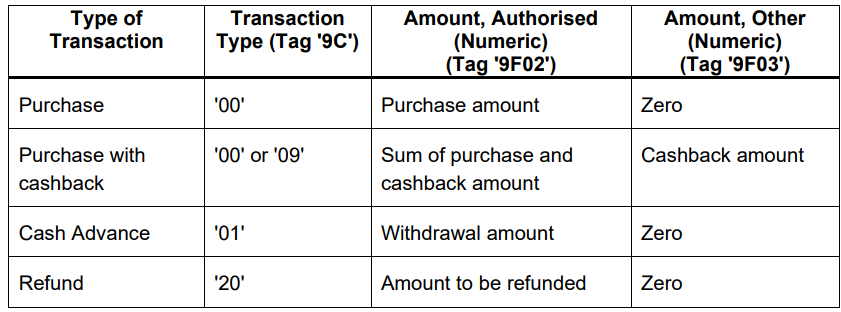
\includegraphics[width=0.8\textwidth]{images/research/transaction_types}
    \caption{\centering Форматы данных для транзакции}
    \label{fig:transaction_types}
\end{figure}


\subsubsection{Этап выбора платежной комбинации}
\label{subsubsec:protocol_activation}

Entry Point выполняет выбор приложения посредством запроса и получения данных от Proximity Payment System Environment (PPSE), встроенного в карту.
Ответ PPSE, возвращаемый картой, содержит один или несколько элементов данных File Control Information (FCI), формирующих список приложений, поддерживаемых картой (в порядке приоритета относительно друг друга) и платежное ядро, с которым они будут работать.
Точка входа сравнивает названия из Application Definition File (ADF) и идентификаторы ядер с набором комбинаций Application Identifier (AID) и Kernel Identifier (тег~-- <<9F2A>>), которые она поддерживает для указанных терминалом типа транзакции, суммы, валюты.
Результатом является список комбинаций, упорядоченных по значению приоритета (для совпадений с равным приоритетом) или по их порядку в списке FCI.
AID и имена ADF можно получить из соответствующих ПС.

Карты большинства ПС не имеют идентификатора ядра в данных FCI, в таком случае Entry Point считывает его отсутствие и выбирает ядро на основе AID следующим образом:
\begin{itemize}
    \item ядро 2 для MasterCard AID,
    \item ядро 3 для Visa AID,
    \item ядро 4 для American Express AID,
    \item ядро 5 для JCB AID,
    \item ядро 6 для Discover AID,
    \item ядро 7 для UnionPay AID.
\end{itemize}

Entry Point выбирает комбинацию с наивысшим приоритетом и отправляет команду SELECT AID с AID этой комбинации и передает обработку выбранному платежному ядру.
После получения ответа на SELECT PPSE может быть выполнена дополнительная фаза процесса выбора приложения, на которой информация о терминале предоставляется карте, что позволяет карте отправить другой список поддерживаемых приложений для использования в процессе выбора приложения.
Поддержка этой дополнительной фазы процесса выбора платежного приложения, включая поддержку команды SEND POI INFORMATION и используемых объектов данных терминала, является необязательной для реализации~\cite{emv_book_B}.

\subsubsection{Этап обработки результата}
\label{subsubsec:outcome_processing}

Результатом обработки платежным ядром является Outcome, представляющий собой команду или указание от платёжного ядра, определяющую дальнейшее поведение терминала, например завершении операции или продолжении обработки посредством вызова онлайн-авторизации.
Каждый Outcome имеет список обязательных параметров на основе которых определяется дальнейшее взаимодействие с картой и ее держателем~\cite{emv_book_A}.

Существует несколько стандартных Outcome:

\begin{itemize}
    \item Select Next~--- <<выполнить поиск следующего доступного платежного ядра или приложения на карте>>, применяется, если текущее ядро не может обработать транзакцию — например, если карта поддерживает несколько платёжных систем;
    \item Try Again~--- <<повторить попытку выполнения операции>>, может быть вызван ошибкой связи или временным сбоем в процессе аутентификации;
    \item Approved~--- <<транзакция одобрена без необходимости онлайн-проверки>>, применяется в случае успешной офлайн-аутентификации и прохождения всех проверок на стороне терминала и карты;
    \item Declined~--- <<транзакция отклонена по одной из причин: неверные данные, превышено количество попыток, карта заблокирована и т.д.>>, используется для завершения транзакции с отказом;
    \item Online Request~--- <<требуется отправки данных на сервер эмитента для онлайн-авторизации>>, используется для установления связи с банком для дополнительной проверки перед одобрением или отклонением транзакции;
    \item Request Online PIN~--- <<требуется ввод PIN-кода с проверкой на сервере эмитента>>, применяется для усиления безопасности, особенно при высоких суммах транзакций;
    \item Try Another Interface~--- <<предложение использовать другой интерфейс для оплаты, используется если текущий способ не позволяет успешно завершить транзакцию, например, из-за ограничений суммы или неисправности NFC;
    \item End Application~--- <<завершение текущего платежного приложения на карте>>, применяется, когда транзакция завершена, либо её невозможно продолжить.
\end{itemize}


% TODO добавить раздел про Online Request
%  есть Remote Authentication в book_E, но это про запрос PIN/подписи и тоже как бы нужно...


%\subsubsection{3DES}
%\subsubsection{MirAccept}
% можно добавить для общей информации, но без понимания принципов их работы можно реализовать рабочую систему



\subsection{Стандарт безопасности PCI DSS}

% TODO: обновить в ТЗ - 6.2.1.1
PCI DSS (Payment Card Industry Data Security Standard)~--- это международный стандарт безопасности, созданный для защиты данных платежных карт и операций, предназначенный для защиты организаций от инцидентов безопасности и обеспечения необходимого уровня защищенности в ПС.
 
Этот стандарт применяется организациями, которые хранят, обрабатывают и передают данные платежных карт.
Платежная деятельность торгово-сервисных предприятий (точек продаж) также должна соответствовать данному стандарту, т.к. они имеют возможность влиять на безопасность данных карт ПС, используемых для оплаты товаров и услуг~\cite{nspk_security}.

Основная задача стандарта — защитить данные Primary Account Number (PAN) и другие конфиденциальные элементы, такие как: PIN-код, коды CVV2/CVC2, данные магнитной полосы, персональные данные держателя карты.

Стандарт состоит из 12 требований , объединённых в 6 контрольных областей :

\begin{enumerate}
    \item построение и поддержание безопасной сети,
    \item защита данных держателей карт,
    \item реализация политик управления доступом,
    \item мониторинг всех действий в системе,
    \item регулярное тестирование контрольных механизмов,
    \item поддержание политики информационной безопасности.
\end{enumerate}

Для достижение безопасности в mPOS-устройствах и мобильных решений оплаты, в соответствии с данным стандартом наиболее важны следующие аспекты:

\begin{itemize}
    \item обеспечение конфиденциальности данных в момент считывания и передачи;
    \item использование защищённых протоколов передачи данных (TLS, HTTPS);
    \item отсутствие хранения PIN-кодов и CVV-кодов в чистом виде;
    \item обеспечение целостности программного обеспечения и защита от несанкционированного изменения кода;
    \item интеграция с системой аудита и журналирования событий.
\end{itemize}

% TODO перепроверить содержимое радела,
%  прочитав https://habr.com/ru/companies/payonline/articles/303330/

\subsection{Формирование требований к системе}

В соответствии с требованиями технического задания аппаратная часть системы осуществляет взаимодействие с бесконтактной платежной картой и передачу полученных в ходе взаимодействия данных на устройство-хост посредством технологии Bluetooth.
Считыватель состоит из Bluetooth-модуль, NFC-модуль и МК, который обеспечивает их работу единую синхронизированную работу.

На основании классификации платежных устройств от ФСБ РФ и ЦБ РФ~\cite{cbr_requirements}, разрабатываемая аппаратная часть системы в совокупности с программой является <<защищенным считывателем карт для пользовательских устройств (SCRP-устройством)>>, т.к. используется вместе с мобильным пользовательским устройством (смартфоном м или планшетом), далее именуется <<считыватель бесконтактных платежных карт>> или <<считыватель>>.

Разрабатываемый считыватель должен разрабатываться на основе требований стандартов EMV и EMV Contactless для последующий возможности последующих сертификаций EMV L1 и EMV Contactless L1 (данные сертификации касаются аппаратной части системы).
Сертификации PCI PTS, EMV L2 и EMV L2 Contactless применимы к ПО, осуществляющему обработку платежных транзакций по стандарту EMV.
Обработку транзакций в разрабатываемой системе осуществляют совместно программа микроконтроллера и приложение на мобильном устройстве, следовательно при разработке мобильного приложения и считывателя должны учитываться требования для данных сертификаций.

Формирование платежной транзакции должна происходить по алгоритму, представленному на рисунке~\ref{fig:kernel_transaction_flow}, адаптированному под выполнение транзакций по картам ПС <<МИР>>, т.е. должен реализовывать обработку в соответствии со спецификацией платежного ядра ПС <<МИР>>~\cite{book_mir}.

Также разрабатываемый считывать имеет тип (Terminal Type по стандарту EMV) 21~--- то есть это торговый терминал, находящийся под контролем ТСП, используемый только для онлайн оплаты с онлайн аутентификацией.
Т.е., для аутентификацию и авторизации необходим обмен данными с эмитентом в режиме реального времени, что реализуется в мобильном приложении  в результате взаимодействия с платежным сервером банка-эквайером посредством выхода Интернет.
Поэтому мобильное приложение должно соответствовать стандарту безопасности PCI DSS Level 1.
Список требований PCI DSS для разрабатываемого мобильного приложения приведен в таблице~\ref{tab:pci_dss_requirements_for_app}.

\begin{longtable}[l]{|P{0.4\textwidth}|P{0.55\textwidth}|}

    \caption{Основные требования PCI DSS, применимые к мобильному приложению}
    \label{tab:pci_dss_requirements_for_app} \\ \hline
    \textbf{Требование PCI DSS} & \textbf{Применение к мобильному приложению} \\ \hline
    \endfirsthead

    \caption*{Продолжение таблицы~\ref{tab:pci_dss_requirements_for_app}} \\ \hline
    \textbf{Требование PCI DSS} & \textbf{Применение к мобильному приложению} \\ \hline
    \endhead

    \endfoot

    \endlastfoot
    1.2 — Контроль за передачей данных & все данные (PAN, токены, статусы) должны передаваться по защищённым каналам связи (TLS, HTTPS) \\
    \hline
    3 — Защита хранящихся данных & запрещено хранить PIN-код, CVV, если требуется временное хранение данных, они должны быть зашифрованы \\
    \hline
    4 — Шифрование передачи данных по открытым сетям & все запросы к серверу должны выполняться через HTTPS с валидированным SSL/TLS-сертификатом \\
    \hline
    6 — Развёртывание обновлений безопасности & приложение должно поддерживать механизм безопасного обновления \\
    \hline
    8 — Управление доступом & аутентификация пользователя обязательна (логин/пароль, биометрия, двухфакторная аутентификация) \\
    \hline
    10 — Журналирование событий & должны сохраняться события: начало транзакции, ошибки, вход в систему, попытки несанкционированного доступа \\
    \hline
    11 — Тестирование контрольных механизмов & необходимо регулярное тестирование на проникновение (pentest), анализ уязвимостей и проверка конфигурации API \\
    \hline
\end{longtable}

Требования пункта 8 зависят от наличия соответствующего функционала в предоставляемом API, требования пункта 11 должны осуществляться со стороны разработчика и правообладателя API.


В результате выполнения анализа предметной области и учета требований технического задания были определены и изучены необходимые технологии для выполнения платежных операций посредством разрабатываемой системы.
Также была изучена актуальная классификация платежных устройств и проанализированы существующие альтернативы разрабатываемой системы: изучены используемые в них программные и аппаратные решения для достижения работы на необходимом уровне безопасности.


